\chapter{Specific requirements}
		\section{External interface requirements}
			\subsection{User interfaces}
				\paragraph{}
					The following mockups give an approximate idea of how the application's interfaces should appear.
				\subsubsection{Unregistered User}
					\paragraph{}
						\begin{center}
						{\small \textbf{Sign-Up}}
						\end{center}
						\vspace{-5mm}
						\begin{figure}[ht]
								\centering
							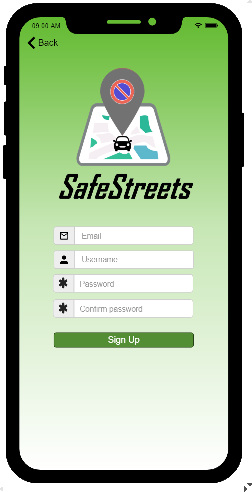
\includegraphics[height=8.8cm] {images/MockUp/User/SignUp.pdf}
								\caption{UU SignUp mockup}
						\end{figure}
				\clearpage
				
				\subsubsection{Registered User}
					\begin{center}
						{\small \textbf{User Login}}
					\end{center}
					\vspace{-5mm}
					\begin{figure}[!h]
						\centering
						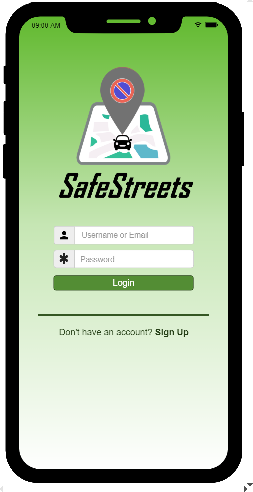
\includegraphics[height=8.5cm]{images/MockUp/User/UserLogin.pdf}
						\caption{User login mockup}
					\end{figure}
					\vspace{-1mm}
					\begin{center}
						{\small \textbf{Get my reports, all reports}}
					\end{center}
					\vspace{-5mm}
					\begin{figure}[!h]
						\centering
						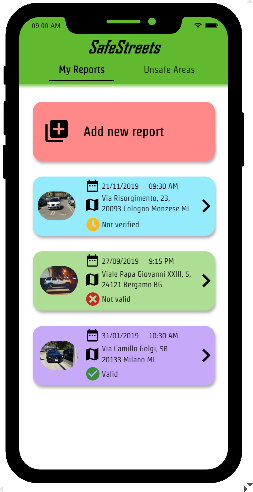
\includegraphics[height=8.5cm]{images/MockUp/User/MyReports.pdf}
						\caption{Get my reports (all) mockup}
					\end{figure}
					\clearpage
					
					\begin{center}
						{\small \textbf{Get my reports, information of a single report}}
					\end{center}
					\vspace{-5mm}
					\begin{figure}[!h]
						\centering
						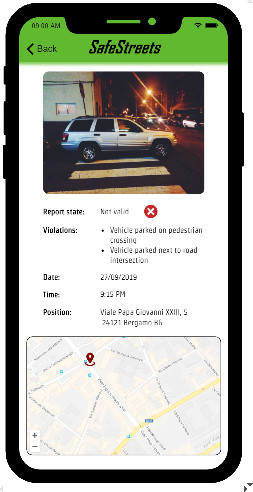
\includegraphics[height=8.5cm]{images/MockUp/User/MyReportExpanded.pdf}
						\caption{Get my reports (detail) mockup}
					\end{figure}
					\vspace{-1mm}
					\begin{center}
						{\small \textbf{Get unsafe areas}}
					\end{center}
					\vspace{-5mm}
					\begin{figure}[!h]
						\centering
						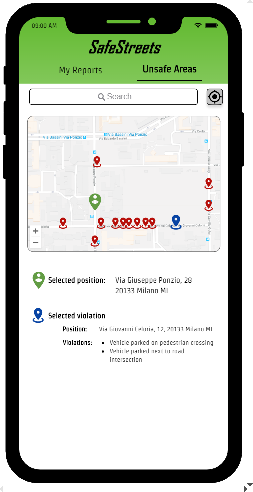
\includegraphics[height=8.5cm]{images/MockUp/User/UnsafeAreas.pdf}
						\caption{Get unsafe areas mockup}
					\end{figure}
					\clearpage
					
					\begin{center}
						{\small \textbf{Add reports, taking picture from camera}}
					\end{center}
					\vspace{-5mm}
					\begin{figure}[!h]
						\centering
						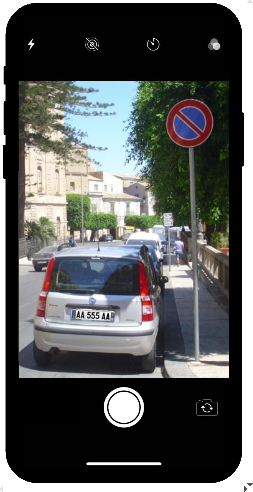
\includegraphics[height=8.5cm]{images/MockUp/User/Report0Camera.pdf}
						\caption{Add report (take picture) mockup}
					\end{figure}
					\vspace{-1mm}
					\begin{center}
						{\small \textbf{Add report, confirmation of taken picture}}
					\end{center}
					\vspace{-5mm}
					\begin{figure}[!h]
						\centering
						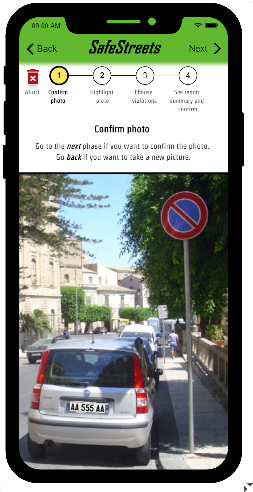
\includegraphics[height=8.5cm]{images/MockUp/User/Report1ConfirmPhoto.pdf}
						\caption{Add report (confirm picture) mockup}
					\end{figure}
					\clearpage
					
					\begin{center}
						{\small \textbf{Add report, highlighting of the vehicle's plate}}
					\end{center}
					\vspace{-5mm}
					\begin{figure}[!h]
						\centering
						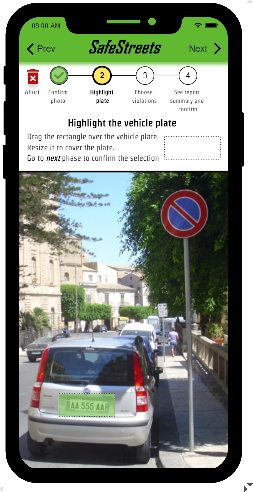
\includegraphics[height=8.5cm]{images/MockUp/User/Report2HighlightPlate.pdf}
						\caption{Add report (highlight plate) mockup}
					\end{figure}
					\vspace{-1mm}
					\begin{center}
						{\small \textbf{Add report, choosing of the violations' type}}
					\end{center}
					\vspace{-5mm}
					\begin{figure}[!h]
						\centering
						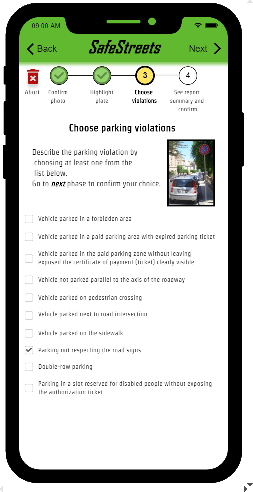
\includegraphics[height=8.5cm]{images/MockUp/User/Report3ChooseViolation.pdf}
						\caption{Get unsafe areas mockup}
					\end{figure}
					\clearpage
					
					\begin{center}
						{\small \textbf{Add report, confirmation}}
					\end{center}
					\vspace{-5mm}
					\begin{figure}[h]
						\centering
						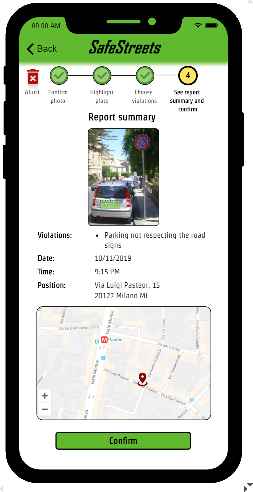
\includegraphics[height=8.5cm]{images/MockUp/User/Report4Confirm.pdf}
						\caption{Add report (confirm) mockup}
						\end{figure}
				\subsubsection{Authority}
					\vspace{-2mm}
					\begin{center}
						{\small \textbf{Authority login}}
					\end{center}
					\vspace{-5mm}
					\begin{figure}[!h]
						\centering
						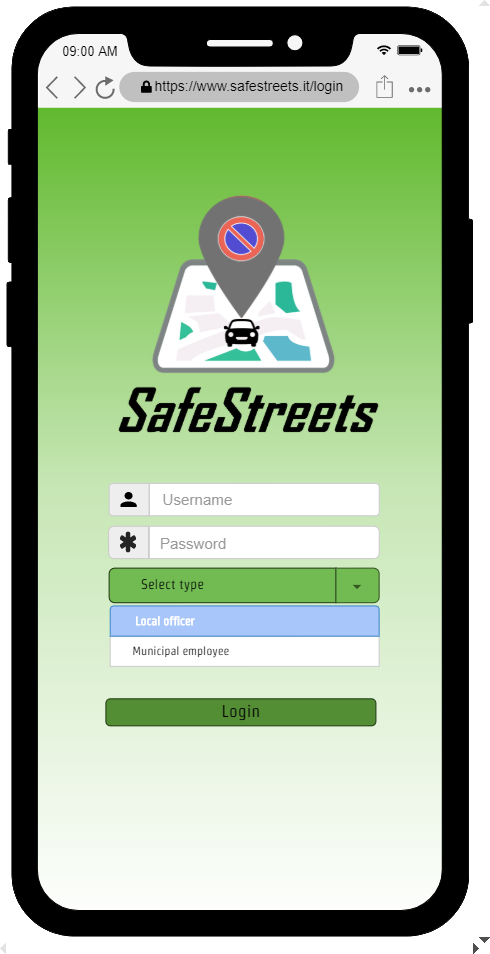
\includegraphics[height=8.5cm]{images/MockUp/Authority/AuthorityLogin.png}
						\caption{Authority login mockup}
						\end{figure}
				\clearpage
				
				\subsubsection{Municipal Employee}
					\begin{center}
						{\small \textbf{Home page}}
					\end{center}
					\vspace{-5mm}
					\begin{figure}[!h]
						\centering
						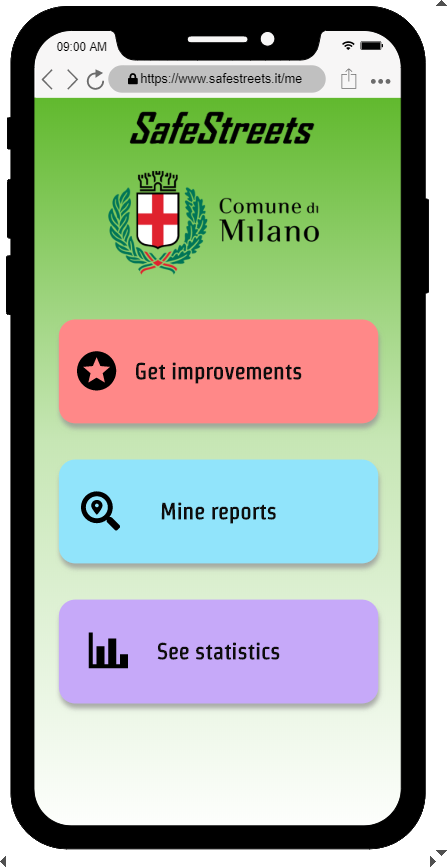
\includegraphics[height=8.5cm]{images/MockUp/Authority/MunicipalEmployee/HomePage.png}
						\caption{Municipal Employee home page mockup}
					\end{figure}
					\vspace{-1mm}
					\begin{center}
						{\small \textbf{Get improvements}}
					\end{center}
					\vspace{-5mm}
					\begin{figure}[!h]
						\centering
						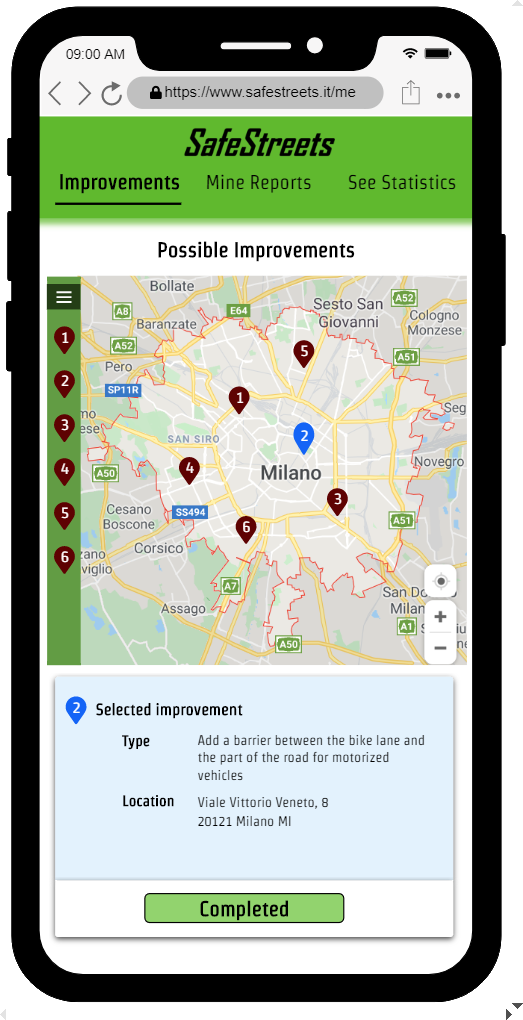
\includegraphics[height=8.5cm]{images/MockUp/Authority/MunicipalEmployee/Improvements.png}
						\caption{Get improvements mockup}
					\end{figure}
					\clearpage
					
					\begin{center}
						{\small \textbf{Mine reports by*}}
					\end{center}
					\vspace{-5mm}
					\begin{figure}[!h]
						\centering
						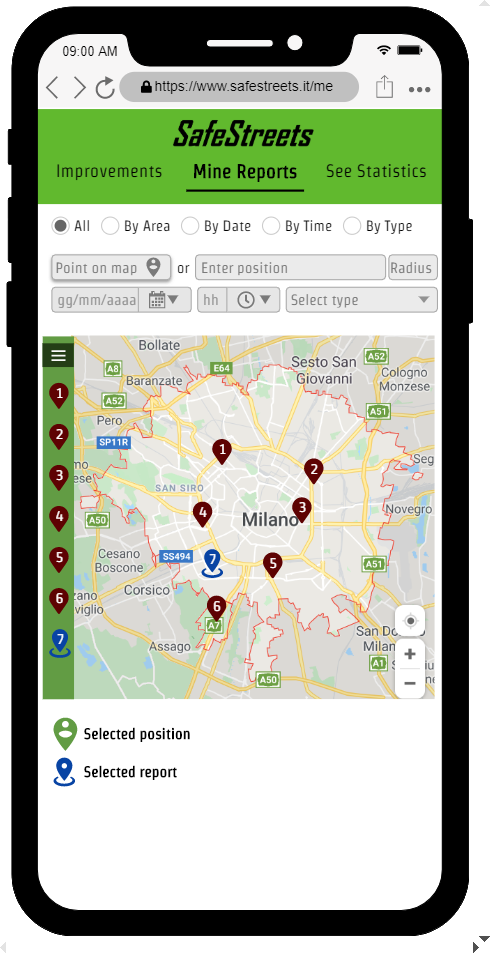
\includegraphics[height=8.5cm]{images/MockUp/Authority/MunicipalEmployee/MineReports.png}
						\caption{Municipal Employee mine reports by* mockup}
					\end{figure}
					\vspace{-1mm}
					\begin{center}
						{\small \textbf{See statistics}}
					\end{center}
					\vspace{-5mm}
					\begin{figure}[!h]
						\centering
						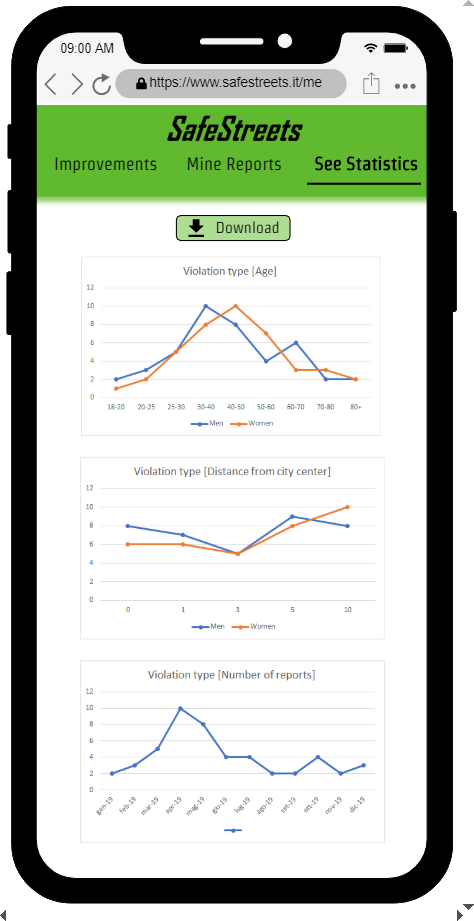
\includegraphics[height=8.5cm]{images/MockUp/Authority/MunicipalEmployee/SeeStatistics.png}
						\caption{See statistics mockup}
					\end{figure}
				\clearpage
				\subsubsection{Local Officer}
				\vspace{-2mm}
				\begin{center}
					{\small \textbf{Home page}}
				\end{center}
				\vspace{-5mm}
				\begin{figure}[!h]
					\centering
					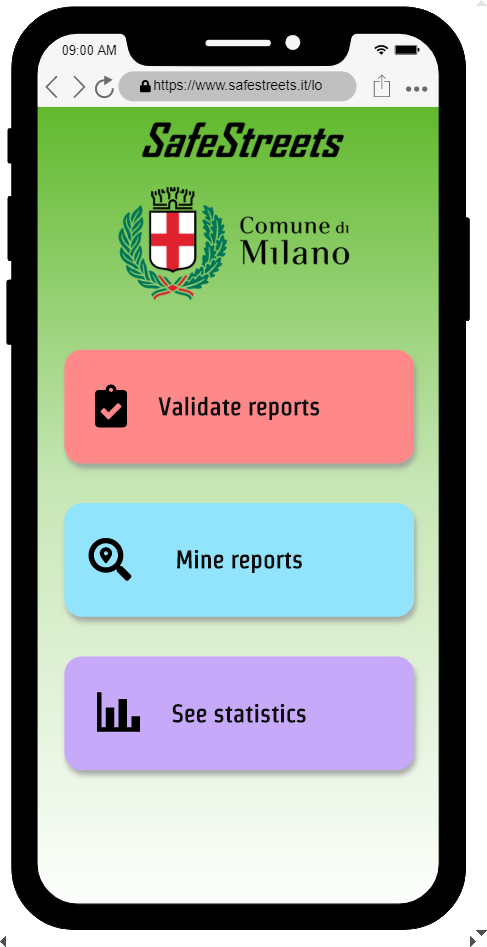
\includegraphics[height=8.5cm]{images/MockUp/Authority/LocalOfficer/HomePage.png}
					\caption{Local Officer home page mockup}
				\end{figure}
				\begin{center}
						{\small \textbf{Validate reports, compact view}}
					\end{center}
					\vspace{-5mm}
					\begin{figure}[!h]
						\centering
						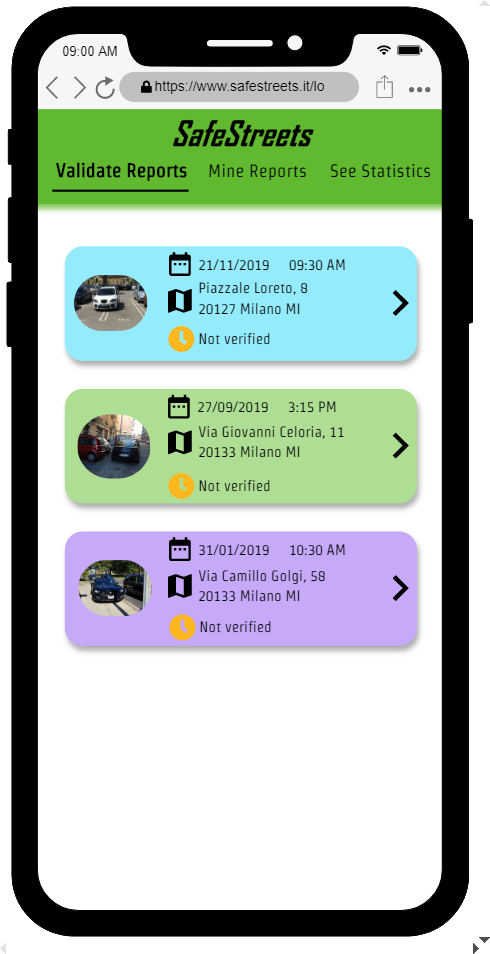
\includegraphics[height=8.5cm]{images/MockUp/Authority/LocalOfficer/ValidateReport.png}
						\caption{Validate reports (all) mockup}
					\end{figure}
					\clearpage
					\vspace{-1mm}
					\begin{center}
						{\small \textbf{Validate report, expanded view}}
					\end{center}
					\vspace{-5mm}
					\begin{figure}[!h]
						\centering
						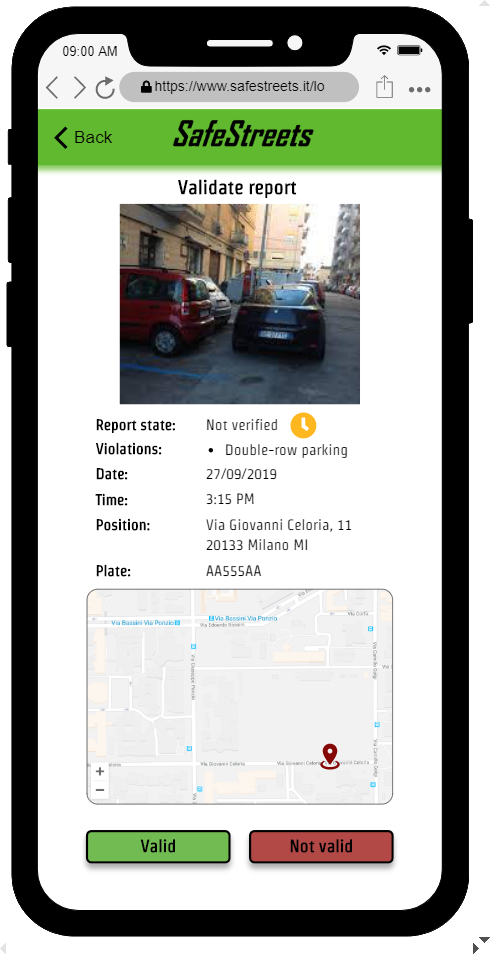
\includegraphics[height=8.5cm]{images/MockUp/Authority/LocalOfficer/ValidateReportExpanded.png}
						\caption{Validate report (detail) mockup}
					\end{figure}
					\vspace{-2mm}
					\begin{center}
						{\small \textbf{Mine reports by*}}
					\end{center}
					\vspace{-5mm}
					\begin{figure}[!h]
						\centering
						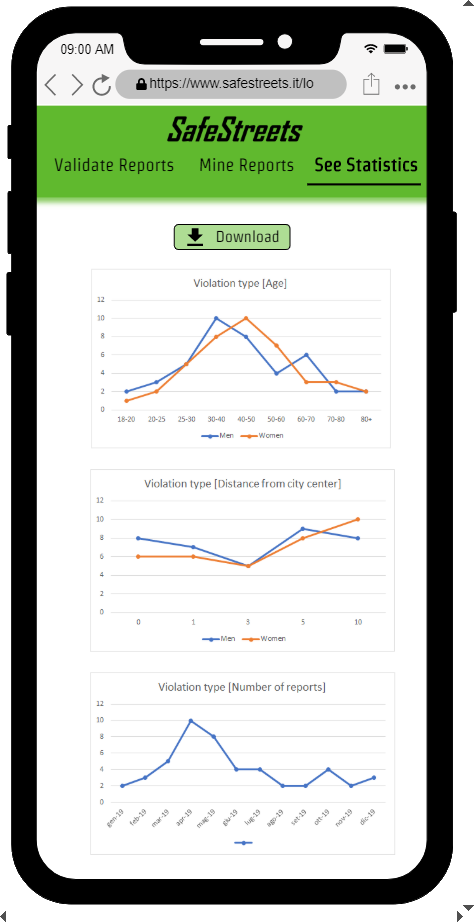
\includegraphics[height=8.5cm]{images/MockUp/Authority/LocalOfficer/SeeStatistics.png}
						\caption{Local Officer mine reports by* mockup}
					\end{figure}
					\clearpage
					\vspace{-2mm}
				\begin{center}
					{\small \textbf{See statistics}}
				\end{center}
				\vspace{-5mm}
				\begin{figure}[!h]
					\centering
					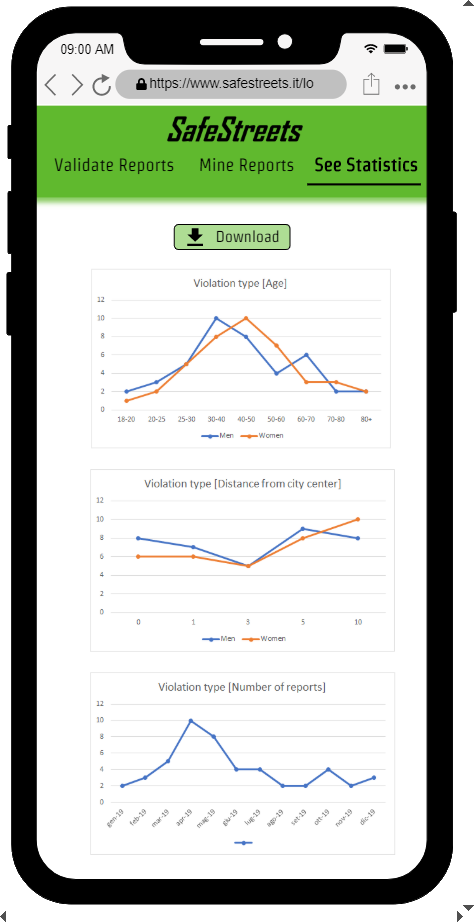
\includegraphics[height=8.5cm]{images/MockUp/Authority/LocalOfficer/SeeStatistics.png}
					\caption{Local Officer see statistics mockup}
				\end{figure}
			\subsection{Hardware interfaces}
				\paragraph{}
					The system has no hardware interface.
			\subsection{Software interfaces}
				\paragraph{}
					The system does not offer any APIs to external applications for its usage.
			\subsection{Communication interfaces}
				\paragraph{}
					The system does not offer any APIs to external applications for communication.
		\section{Functional requirements}
			\subsection{Scenarios}
				\subsubsection{Scenario 1}
					\paragraph{}
						Cat has a disabled child. Tired from everybody that leaves their car in the disable's parking lot, Cat decides to download and install the SafeStreets app. After subscribing to the service, she starts to take pictures of all the perpetrator's cars. Some time after, Cat notices that her reports are getting validated and along with that the number of times that she founds cars in the disabled parking lot starts to diminish, that may be because the local police intervened and ticketed them.
				\subsubsection{Scenario 2}
					\paragraph{}
						Ned is looking for a house in the city, he has always lived in the countryside and he's scared of the possibility to live in areas with difficulty in finding car parks. He opens SafeStreets and using ''Get unsafe areas'' and, by selecting areas around his favourite house on sale, he can find what happened there and he can avoid the worst areas, looking for a house with confidence.
				\subsubsection{Scenario 3}
					\paragraph{}
						Jon has a reputation for not being a trustworthy guy. When he decides to use SafeStreets, Jon starts to report every car that he does not like, hoping that the owners of those car will receive a ticket. Luckily for the owners, those report won't incur in any fine because the local police is able to validate the received reports and does not issue the cars in order, ignoring Jon's report.
				\subsubsection{Scenario 4}
					\paragraph{}
						Martha works as a municipal employee. The mayor asks her to make a list of all possible investment to develop the streets of the city, in order to increase street security. Luckily for Martha, SafeStreets with its function ''Get Improvements'', highlights the most unsafe areas and suggests possible interventions. Reading these recommendations, Martha realizes that some of them have already been done so she diligently set them as completed. Martha can now finish her assignment quickly.
				\subsubsection{Scenario 5}
					\paragraph{}
						The mayor, to promote his image before the next elections, wants to publish a report with the statistics regarding public security. With SafeStreets his secretary can easily retrieve such information and prepare a detailed report with all the statistics about how public street security has improved during the mayor's mandate.
				\subsubsection{Scenario 6}
					\paragraph{}
						A group of citizens is concerned with the street security of their neighborhood but they don't have any real data that can be used to support their concerns. They go to the municipality to ask for more information and possibly an intervention of the authorities. The municipality can quickly search for data regarding their area and forward it to higher authorities that will hopefully do something.
				\subsubsection{Scenario 7}
					\paragraph{}
						A local officer in patrol is tasked to give fines during his work shift but usually, this isn't such an easy task. Normally he would spend a lot of time searching the usual street but, using SafeStreets, he can now retrieve reports about positions of parking violations using ''Mine Reports'' function. With this information, the local officer starts the search. Luckily for him, he finds a lot of violations in the streets specified by SafeStreet, so he can proceed and charge the owners of those cars for their sins (violations).
			\clearpage
			\subsection{Use case diagrams}
				\subsubsection{Unregistered User}
					\begin{figure}[!h]
						\centering
						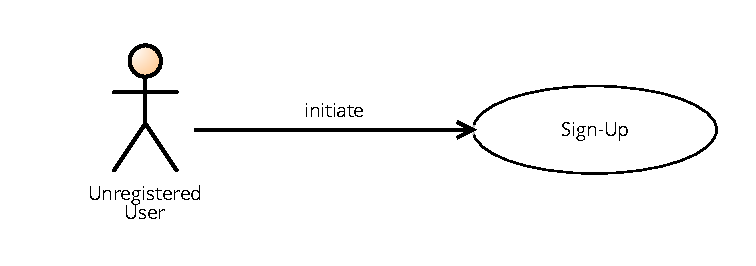
\includegraphics[width=\textwidth]{images/UseCase/UU.pdf}
						\caption{Unregisterd User use case diagram}
					\end{figure}
				\subsubsection{Registered User}
					\begin{figure}[!h]
						\centering
						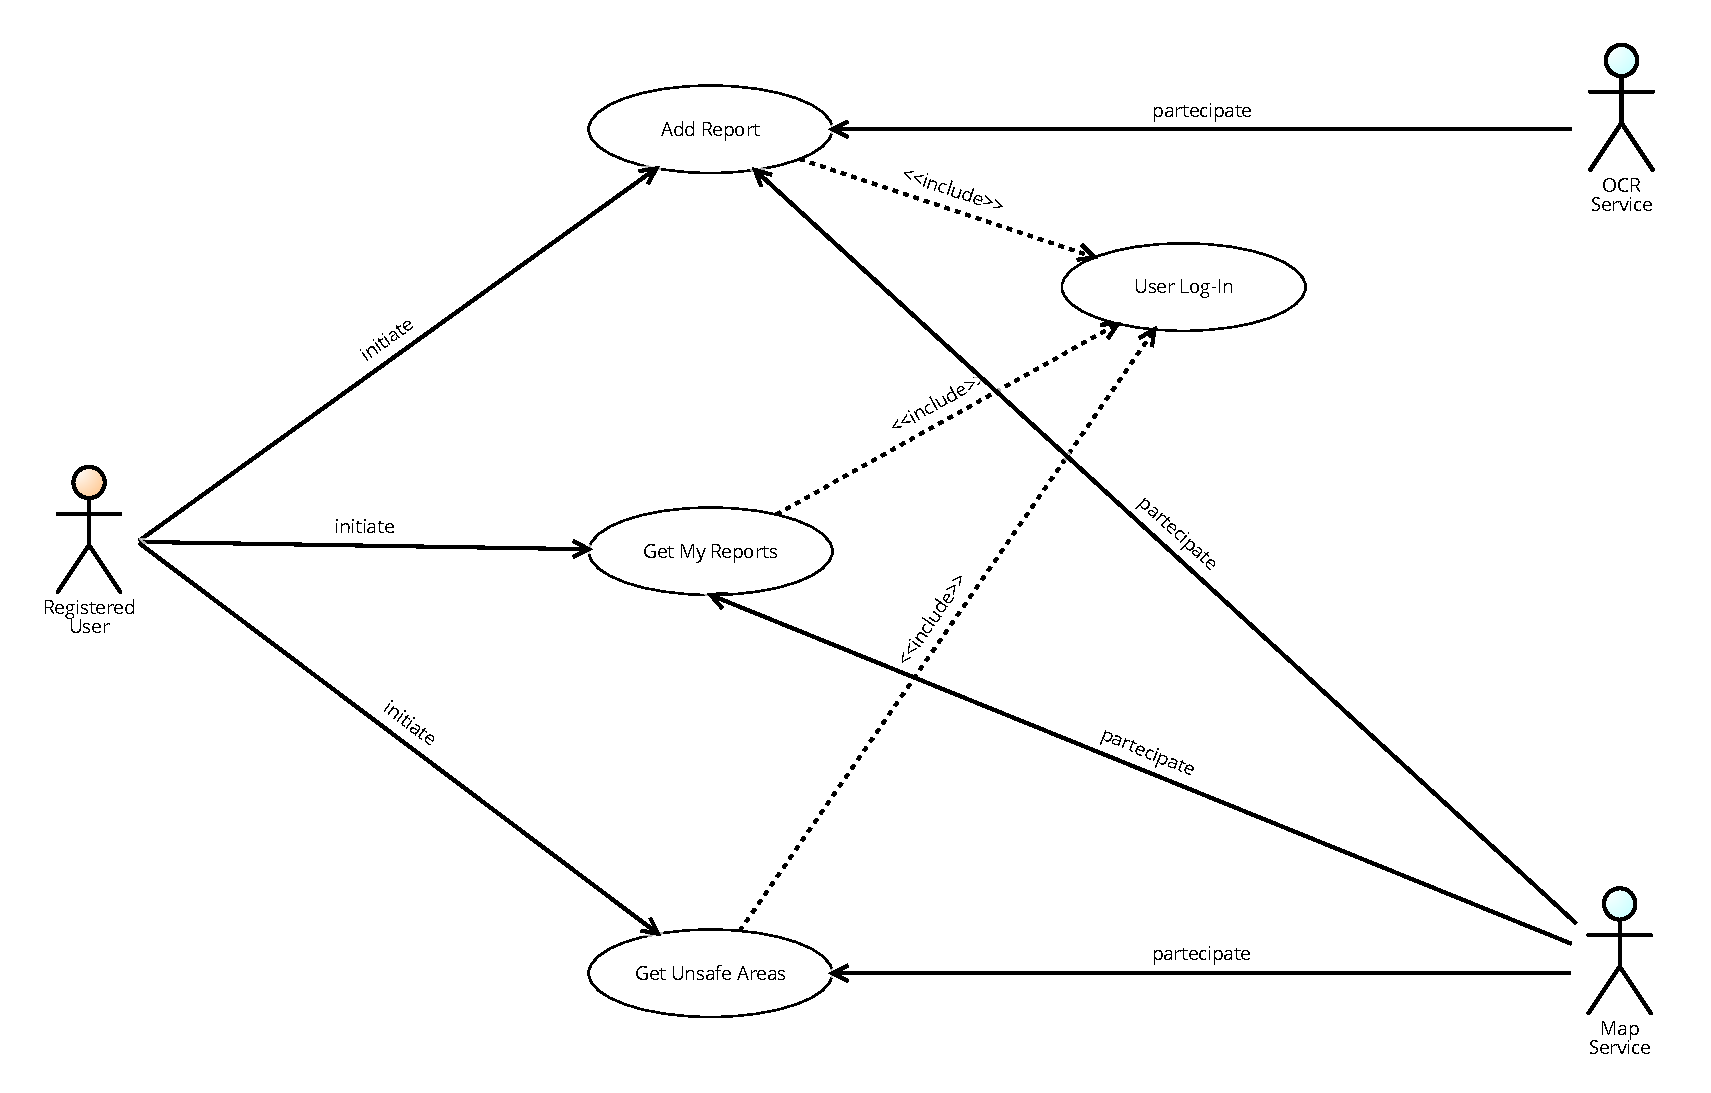
\includegraphics[width=\textwidth]{images/UseCase/RU.pdf}
						\caption{Registered User use case diagram}
					\end{figure}
				\clearpage
				\subsubsection{Municipal Employee}
					\vspace{-7mm}
					\begin{figure}[!h]
						\centering
						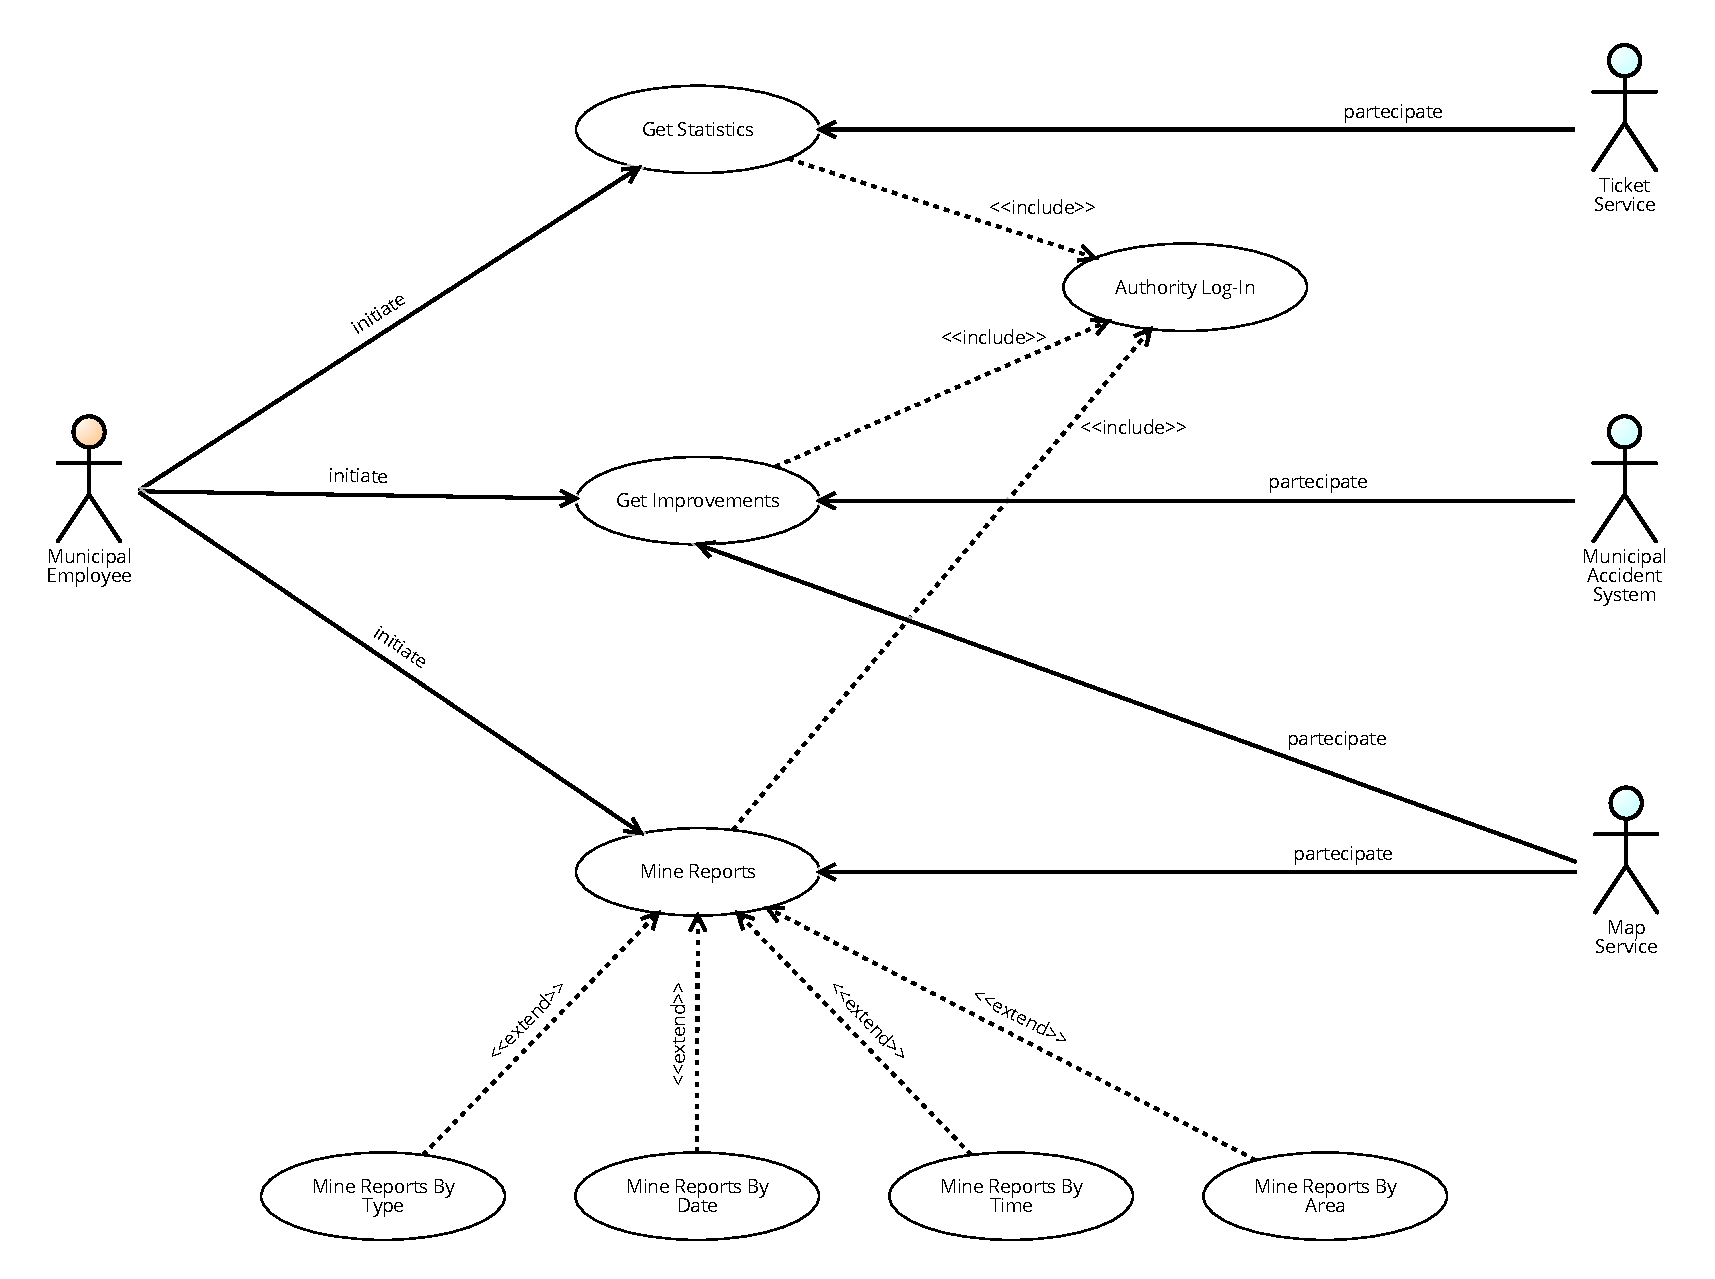
\includegraphics[width=\textwidth]{images/UseCase/ME.pdf}
						\caption{Municipal Employee use case diagram}
					\end{figure}
				\subsubsection{Local Officer}
				\vspace{-7mm}
					\begin{figure}[!h]
						\centering
						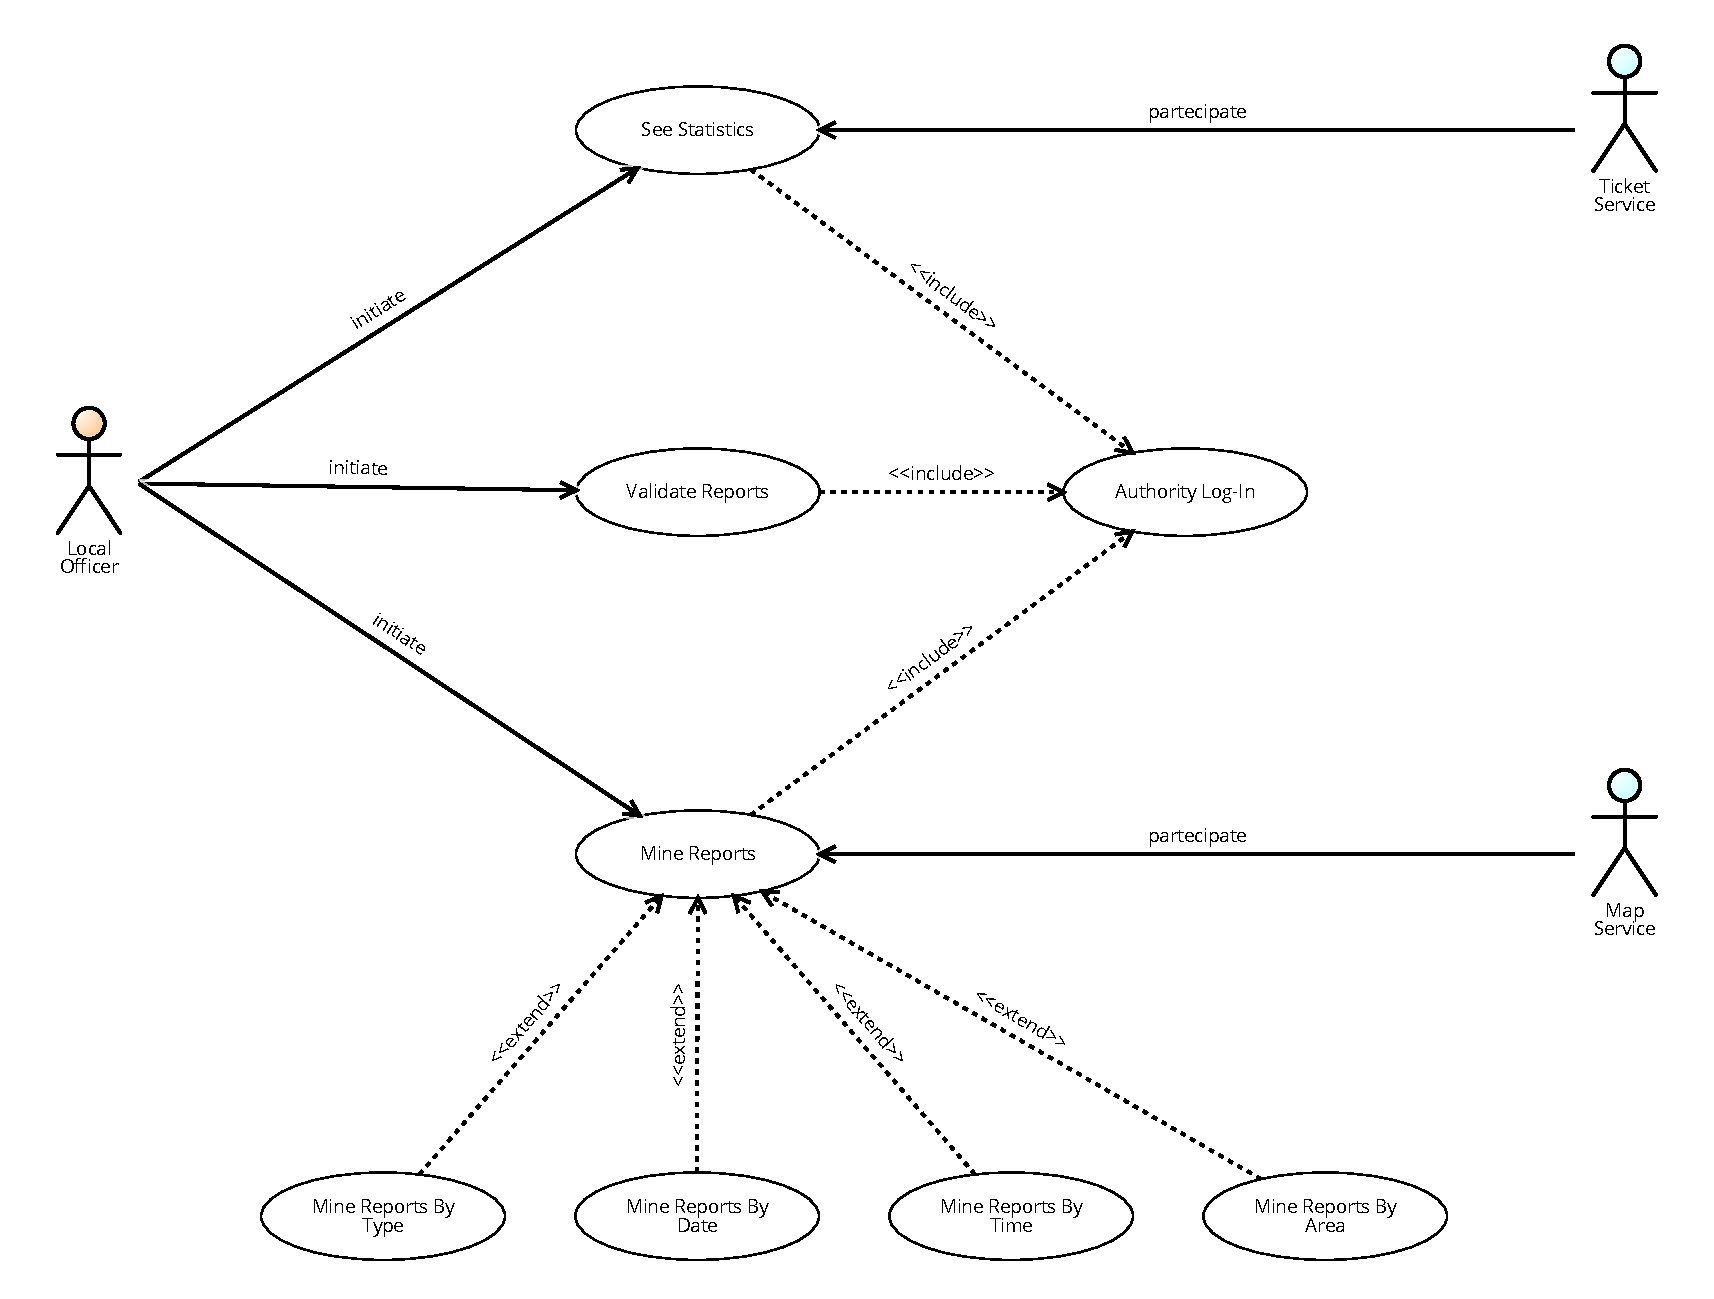
\includegraphics[width=\textwidth]{images/UseCase/LO.pdf}
						\caption{Local Officer use case diagram}
					\end{figure}
			\clearpage
			\subsection{Use cases}
				\subsubsection{Sign-Up}
					\begin{table}[!h]
						\centering
						\begin{tabular}{lp{0.6\textwidth}}
							\toprule
							\textbf{Name} & \textbf{Sign-Up} \\[1mm]
							\midrule
							\textbf{Actors} & Unregistered User \\[1mm]
							\textbf{Entry Conditions} & The UU is already on the login page. \vspace{1mm}\\
							\textbf{Event Flow} &
							\vspace{-5mm} 
							\begin{enumerate}
								\setlength\itemsep{0.5mm}
								\item The UU clicks on the ''Sign-Up'' field to start the registration process
								\item The UU provides his/her email address
								\item The UU provides a username
								\item The UU provides a password and writes it again for confirmation
								\item The UU clicks on the confirmation button
								\item The system saves the data
							\end{enumerate} \\
							\textbf{Exit Conditions} & The UU becomes now a RU. From now on he/she can log into the  application and use SafeStreets service. \vspace{1mm}\\
							
							\textbf{Exceptions} &
							\vspace{-5mm} 
							\begin{enumerate}
								\item The UU provides an already used email address
								\item The UU provides an already used username
								\item The two passwords provided by the UU are not correspoding
							\end{enumerate}
							\vspace{-7mm}
							\paragraph{}
								In the case 1 an error message is displayed, saying ''Credentials already in use,  please log in'', and the UU is taken back to the login page.
							\paragraph{}
							\vspace{-4mm}
								In the case 2 an error message is displayed, saying ''Username already in use, please choose a different one'', and the UU is taken back to the point 2.
							\paragraph{}
							\vspace{-4mm}
								In the case 3 an error message is displayed, saying ''Email already in use, please log in'', and the UU is taken back to the login page. \\[1mm]
							\bottomrule
						\end{tabular}
						\caption{Sign up use case}
					\end{table}
					\clearpage
					\vspace{-7mm}
					\subsubsection{Registered User login}
					\begin{table}[!h]
						\centering
						\vspace{-5mm}
						\begin{tabular}{lp{0.679\textwidth}}
							\toprule
							\textbf{Name} & \textbf{Registered User login} \\[1mm]
							\midrule
							\textbf{Actors} & Registered User \\[1mm]
							\textbf{Entry Conditions} & The RU is already on the login page \vspace{1mm}\\
							\textbf{Event Flow} &
							\vspace{-5mm} 
							\begin{enumerate}
								\setlength\itemsep{0.2mm}
								\item The RU provides his/her username or email.
								\item The RU provides his/her password.
								\item The RU clicks on the confirmation button
								\item The system redirects the RU to the corresponding home page.
							\end{enumerate} \\
							\textbf{Exit Conditions} & The RU is successfully redirected to the corresponding home page. \vspace{1mm}\\
							\textbf{Exceptions} &
							\vspace{-5mm} 
							\begin{enumerate}
								\item The RU provides an incorrect username, email or password.
							\end{enumerate}
							\vspace{-7mm}
							\paragraph{}
								In the case 1 an error message is displayed, saying "Wrong Credentials", and the RU is taken
back to the point 1. \\[1mm]
							\bottomrule
						\end{tabular}
						\caption{Registered User login use case}
					\end{table}
					\vspace{-7.5mm}
					\subsubsection{Add report}
					\begin{table}[!h]
						\centering
						\vspace{-4.5mm}
						\begin{tabular}{lp{0.679\textwidth}}
							\toprule
							\textbf{Name} & \textbf{Add report} \\[1mm]
							\midrule
							\textbf{Actors} & Registered User, OCR Service, Map Service\\[1mm]
							\textbf{Entry Conditions} & The RU has logged in and is in the home page, which is the ''Get My Reports'' page \vspace{1mm}\\
							\textbf{Event Flow} &
							\vspace{-5mm} 
							\begin{enumerate}
								\setlength\itemsep{0.1mm}
								\item The RU clicks on the ''Add Report'' button.
								\item The RU takes a photo of the vehicle through his/her device's camera and confirms the picture
								\item The RU highlights the plate of the reported vehicle and goes to the next phase.
								\item The RU adds one or more type of violations and confirms.
								\item The RU sees the complete report and confirms.
								\item The system receives the report and stores it, with the eventual plate recognized thanks to the OCRS.
							\end{enumerate} \\				
							\textbf{Exit Conditions} & The RU successfully uploads a new report into the system. Then he/she is taken back to the home page.\vspace{1mm}\\
							\textbf{Exceptions} & There are no exceptions under the given domain assumptions. \\[1mm]
							\bottomrule
						\end{tabular}
						\caption{Add report use case}
					\end{table}
					\clearpage
					\subsubsection{Get my reports}
					\begin{table}[!h]
						\centering
						\vspace{-4mm}
						\begin{tabular}{lp{0.679\textwidth}}
							\toprule
							\textbf{Name} & \textbf{Get my reports} \\[1mm]
							\midrule
							\textbf{Actors} & Registered User, Map Service \\[1mm]
							\textbf{Entry Conditions} & The RU has logged in and is in the home page, which is "Get My Reports" page. \vspace{1mm}\\
							\textbf{Event Flow} &
							\vspace{-5mm} 
							\begin{enumerate}
								\setlength\itemsep{0.2mm}
								\item The system automatically provides the RU with the reports he/she has sent, sorted in chronological order, starting from the newest one, preceded by the "Add Report" button.
								\item Eventually the RU is able to open a report, see all its information, with the position provided by the MS, and see its status.
							\end{enumerate} \\
							\textbf{Exit Conditions} & The RU successfully gets his/her reports and is able to navigate through them. \vspace{2mm}\\
							\textbf{Exceptions} &
							\vspace{-5mm} 
							\begin{enumerate}
								\item The RU has never uploaded any report
							\end{enumerate}
							\vspace{-7mm}
							\paragraph{}
								The case 1 is handled by showing only the "Add Report" button. \\
							\bottomrule
						\end{tabular}
						\caption{Get my reports use case}
					\end{table}
					\subsubsection{Get unsafe areas}
					\begin{table}[!h]
						\centering
						\vspace{-4mm}
						\begin{tabular}{lp{0.679\textwidth}}
							\toprule
							\textbf{Name} & \textbf{Get unsafe areas} \\[1mm]
							\midrule
							\textbf{Actors} & Registered User, Map Service \\[1mm]
							\textbf{Entry Conditions} &The RU has logged in and is in the home page, which is the "Get My Reports" page. \vspace{1mm}\\
							\textbf{Event Flow} &
							\vspace{-5mm} 
							\begin{enumerate}
								\setlength\itemsep{0.2mm}
								\item The RU has to swipe to the "Unsafe areas" page.
								\item Once in the correct page, the RU has to provide an address or use his/her current GPS location
								\item A map with the violations, shown as points, is displayed. The map is provided by the MS
							\end{enumerate} \\
							\textbf{Exit Conditions} & The RU now is able to browse on the map between violations and see their type. \vspace{1mm}\\
							\textbf{Exceptions} & 
								\vspace{-5mm} 
								\begin{enumerate}
									\item The RU provides an invalid address
								\end{enumerate}
								\vspace{-7mm}
								\paragraph{}
									In the case 1 an error message is displayed, saying "Invalid address", and the RU is taken back to the point 2. \\
							\bottomrule
						\end{tabular}
						\caption{Get unsafe areas use case}
					\end{table}
					\clearpage
					\subsubsection{Authority login}
					\begin{table}[!h]
						\centering
						\vspace{-4mm}
						\begin{tabular}{lp{0.679\textwidth}}
							\toprule
							\textbf{Name} & \textbf{Authority login} \\[1mm]
							\midrule
							\textbf{Actors} & Municipal Employee, Local Officer \\[1mm]
							\textbf{Entry Conditions} & The ME/LO is already on the login page. \vspace{1mm}\\
							\textbf{Event Flow} &
							\vspace{-5mm} 
							\begin{enumerate}[noitemsep]
								\item The ME/LO provides his/her username.
								\item The ME/LO provides his/her password.
								\item The ME/LO chooses his/her type: "Municipal Employee" or "Local Officer".
								\item The ME/LO clicks on the confirmation button.
								\item The system redirects the ME/LO to the corresponding home page.
							\end{enumerate} \\
							\textbf{Exit Conditions} & The ME/LO is successfully redirected to the home page. \vspace{2mm}\\
							\textbf{Exceptions} &
							\vspace{-5mm} 
							\begin{enumerate}
								\item The ME/LO provides an incorrect username or password.
							\end{enumerate}
							\vspace{-7mm}
							\paragraph{}
								In the case 1 an error message is displayed, saying "Invalid credentials", and the ME/LO is taken back to the point 1. \\
							\bottomrule
						\end{tabular}
						\caption{Authority login use case}
					\end{table}
					\vspace{-7mm}
					\subsubsection{See statistics}
					\begin{table}[!h]
						\centering
						\vspace{-4mm}
						\begin{tabular}{lp{0.679\textwidth}}
							\toprule
							\textbf{Name} & \textbf{See statistics} \\[1mm]
							\midrule
							\textbf{Actors} & Municipal Employee, Local Officer, Ticket Service \\[1mm]
							\textbf{Entry Conditions} & The ME/LO has logged in and is in the home page. \vspace{1mm}\\
							\textbf{Event Flow} &
							\vspace{-5mm} 
							\begin{enumerate}
								\setlength\itemsep{0.1mm}
								\item The ME/LO clicks on the "See Statistics".
								\item The system creates statistics using stored valid reports and issued tickets from Ticket Service.
								\item The system sends the statistics to the ME/LO.
								\item The ME/LO chooses the type of statistics to retrieve.
								\item The ME/LO can see and download the received statistics.
							\end{enumerate} \\
							\textbf{Exit Conditions} & The ME/LO successfully receives the statistics provided by the system. \vspace{1mm}\\
							\textbf{Exceptions} & 
								\vspace{-5mm} 
								\begin{enumerate}
									\item The system has no data to build statistics on.
								\end{enumerate}
								\vspace{-7mm}
								\paragraph{}
									In the case 1 an error message is displayed, saying "There is not enough data to create statistics", and the ME is taken back to the home page.\\
							\bottomrule
						\end{tabular}
						\caption{See statistics use case}
					\end{table}
					
					
					\clearpage
					\subsubsection{Get improvements}
					\begin{table}[!h]
						\centering
						\vspace{-2mm}
						\begin{tabular}{lp{0.679\textwidth}}
							\toprule
							\textbf{Name} & \textbf{Get improvements} \\[1mm]
							\midrule
							\textbf{Actors} & Municipal Employee, Municipal Accident Service, Map Service \\[1mm]
							\textbf{Entry Conditions} & The ME has logged in and is in the home page. \vspace{1mm}\\
							\textbf{Event Flow} &
							\vspace{-5mm} 
							\begin{enumerate}
								\setlength\itemsep{0.2mm}
								\item The ME clicks on the "Get Improvements" function.
								\item The system cross its information with the MAS and finds all the possible improvements in the ME's municipality.
								\item The system sends the information to the ME.
								\item The possible improvements are shown in a descendant list on the left, starting from the most urgent one. A map with the possible improvements, shown as points, is displayed on the right, thanks to the MS.
								\item The ME can click on a improvements and see it highlighted on the map and see its detail below.
							\end{enumerate} \\
							\textbf{Exit Conditions} & The ME can browse through all the possible improvements in his/her municipality. \vspace{1mm}\\
							\textbf{Exceptions} & 
								\vspace{-5mm} 
								\begin{enumerate}
									\item There are no possible improvements.
								\end{enumerate}
								\vspace{-7mm}
								\paragraph{}
									In the case 1 an error message is displayed, saying "There is not enough data to generate improvements", and the ME/LO is taken back to the home page. \\
							\bottomrule
						\end{tabular}
						\caption{Get improvements use case}
					\end{table}
					\clearpage
					\subsubsection{Mine reports by all}
					\begin{table}[!h]
						\centering
						\vspace{-2mm}
						\begin{tabular}{lp{0.679\textwidth}}
							\toprule
							\textbf{Name} & \textbf{Mine reports by all} \\[1mm]
							\midrule
							\textbf{Actors} & Municipal Employee, Local Officer, Map Service \\[1mm]
							\textbf{Entry Conditions} & The ME/LO has logged in and is in the home page. \vspace{1mm}\\
							\textbf{Event Flow} &
							\vspace{-5mm} 
							\begin{enumerate}
								\setlength\itemsep{0.2mm}
								\item The ME/LO clicks on the "Mine Reports" function.
								\item The ME/LO chooses the "Mine By All" option.
								\item The system provides the ME/LO with all the violations in his/her municipality.
								\item Only the violation types are shown, in a list on the left, starting from the newest one. A map with violation types, shown as points, is displayed on the right, thanks to the MS.
							\end{enumerate} \\
							\textbf{Exit Conditions} & The ME/LO is able to search through the violations and see where and when they happened. \vspace{1mm}\\
							\textbf{Exceptions} & 
								\vspace{-5mm} 
								\begin{enumerate}
									\item There are no reports for the ME/LO municipality.
								\end{enumerate}
								\vspace{-7mm}
								\paragraph{}
									In the case 1 an error message is displayed, saying "There are no Violations to be displayed", and the ME/LO is taken back to the home page. \\
							\bottomrule
						\end{tabular}
						\caption{Mine reports by all use case}
					\end{table}
					\clearpage
					\subsubsection{Mine reports by type}
					\begin{table}[!h]
						\centering
						\vspace{-2mm}
						\begin{tabular}{lp{0.679\textwidth}}
							\toprule
							\textbf{Name} & \textbf{Mine reports by type} \\[1mm]
							\midrule
							\textbf{Actors} & Municipal Employee, Local Officer, Map Service \\[1mm]
							\textbf{Entry Conditions} & The ME/LO has logged in and is in the home page. \vspace{1mm}\\
							\textbf{Event Flow} &
							\vspace{-5mm} 
							\begin{enumerate}
								\setlength\itemsep{0.2mm}
								\item The ME/LO clicks on the "Mine Reports" function.
								\item The ME/LO chooses the "Mine By Type" option.
								\item The ME/LO decides one or more types of violations to retrieve.
								\item The system provides the ME/LO with all the violations in his/her municipality, with at least one of the given types.
								\item Only the violation types are shown, in a list on the left, starting from the newest one. A map with violation types, shown as points, is displayed on the right, thanks to the MS.
							\end{enumerate} \\
							\textbf{Exit Conditions} & The ME/LO is able to search through the violations and see where and when they happened. \vspace{1mm}\\
							\textbf{Exceptions} & 
								\vspace{-5mm} 
								\begin{enumerate}
									\item There are no reports with at least one of the given violation type.
								\end{enumerate}
								\vspace{-7mm}
								\paragraph{}
									In the case 1 an error message is displayed, saying "There are no Violations to be displayed", and the ME/LO is taken back to the home page. \\
							\bottomrule
						\end{tabular}
						\caption{Mine reports by type use case}
					\end{table}
					\clearpage
					\subsubsection{Mine reports by date}
					\begin{table}[!h]
						\centering
						\vspace{-2mm}
						\begin{tabular}{lp{0.679\textwidth}}
							\toprule
							\textbf{Name} & \textbf{Mine reports by date} \\[1mm]
							\midrule
							\textbf{Actors} & Municipal Employee, Local Officer, Map Service \\[1mm]
							\textbf{Entry Conditions} & The ME/LO has logged in and is in the home page. \vspace{1mm}\\
							\textbf{Event Flow} &
							\vspace{-5mm} 
							\begin{enumerate}
								\setlength\itemsep{0.2mm}
								\item The ME/LO clicks on the "Mine Reports" function.
								\item The ME/LO chooses the "Mine By Date" option.
								\item The ME/LO decides the specific date of the violations to retrieve.
								\item The system provides the ME/LO with all the violations in his/her municipality that were issued in the specific day.
								\item Only the violation types are shown, in a list on the left. A map with violation types, shown as points, is displayed on the right, thanks to the MS.
							\end{enumerate} \\
							\textbf{Exit Conditions} & The ME/LO is able to search through the violations and see where they happened. \vspace{1mm}\\
							\textbf{Exceptions} & 
								\vspace{-5mm} 
								\begin{enumerate}
									\item There are no reports issued in the specific date.
								\end{enumerate}
								\vspace{-7mm}
								\paragraph{}
									In the case 1 an error message is displayed, saying "There are no Violations to be displayed", and the ME/LO is taken back to the home page. \\
							\bottomrule
						\end{tabular}
						\caption{Mine reports by date use case}
					\end{table}
					\clearpage
					\subsubsection{Mine reports by time}
					\begin{table}[!h]
						\centering
						\vspace{-2mm}
						\begin{tabular}{lp{0.679\textwidth}}
							\toprule
							\textbf{Name} & \textbf{Mine reports by time} \\[1mm]
							\midrule
							\textbf{Actors} & Municipal Employee, Local Officer, Map Service \\[1mm]
							\textbf{Entry Conditions} & The ME/LO has logged in and is in the home page. \vspace{1mm}\\
							\textbf{Event Flow} &
							\vspace{-5mm} 
							\begin{enumerate}
								\setlength\itemsep{0.2mm}
								\item The ME/LO clicks on the "Mine Reports" function.
								\item The ME/LO chooses the "Mine By Time" option.
								\item The ME/LO decides the time (expressed in hours, i.e. 8 pm) for the violations he/she wants to retrieve.
								\item The system provides the ME/LO with all the violations in his/her municipality that were issued at the specific time.
								\item Only the violation types are shown, in a list on the left. A map with violation types, shown as points, is displayed on the right, thanks to the MS.
							\end{enumerate} \\
							\textbf{Exit Conditions} & The ME/LO is able to search through the violations and see where they happened. \vspace{1mm}\\
							\textbf{Exceptions} & 
								\vspace{-5mm} 
								\begin{enumerate}
									\item There are no reports issued at the specific time.
								\end{enumerate}
								\vspace{-7mm}
								\paragraph{}
									In the case 1 an error message is displayed, saying "There are no Violations to be displayed", and the ME/LO is taken back to the home page. \\
							\bottomrule
						\end{tabular}
						\caption{Mine reports by time use case}
					\end{table}
					\clearpage
					\subsubsection{Mine reports by area}
					\begin{table}[!h]
						\centering
						\vspace{-2mm}
						\begin{tabular}{lp{0.679\textwidth}}
							\toprule
							\textbf{Name} & \textbf{Mine reports by area} \\[1mm]
							\midrule
							\textbf{Actors} & Municipal Employee, Local Officer, Map Service \\[1mm]
							\textbf{Entry Conditions} & The ME/LO has logged in and is in the home page. \vspace{1mm}\\
							\textbf{Event Flow} &
							\vspace{-5mm} 
							\begin{enumerate}
								\setlength\itemsep{0.2mm}
								\item The ME/LO clicks on the "Mine Reports" function.
								\item The ME/LO chooses the "Mine By Area" option.
								\item The ME/LO decides the address, or selects a point on a map provided by the MS, of the violations to retrieve and select the radius of the search.
								\item The system provides the ME/LO with all the violations in his/her municipality that were issued within the specified radius.
								\item Only the violation types are shown, in a list on the left, starting from the newest one. A map with violation types, shown as points, is displayed on the right, thanks to the MS.
							\end{enumerate} \\
							\textbf{Exit Conditions} & The ME/LO is able to search through the violations and see when they happened. \vspace{1mm}\\
							\textbf{Exceptions} & 
								\vspace{-5mm} 
								\begin{enumerate}
									\item There are no reports issued in the specific area.
								\end{enumerate}
								\vspace{-7mm}
								\paragraph{}
									In the case 1 an error message is displayed, saying "There are no Violations to be displayed", and the ME/LO is taken back to the home page. \\
							\bottomrule
						\end{tabular}
						\caption{Mine reports by area use case}
					\end{table}
					\clearpage
					\subsubsection{Validate reports}
					\begin{table}[!h]
						\centering
						\vspace{-2mm}
						\begin{tabular}{lp{0.679\textwidth}}
							\toprule
							\textbf{Name} & \textbf{Validate reports} \\[1mm]
							\midrule
							\textbf{Actors} & Local Officer, Ticket Service \\[1mm]
							\textbf{Entry Conditions} & The LO has logged in and is in the home page. \vspace{1mm}\\
							\textbf{Event Flow} &
							\vspace{-5mm} 
							\begin{enumerate}
								\setlength\itemsep{0.2mm}
								\item The LO clicks on the "Validate Report" function.
								\item The system provides the LO with all the reports of his/her municipality still not verified.
								\item The reports are shown starting from the newest one.
								\item The LO clicks on one report and is able to validate or invalidate it.
								\item Eventually the LO can use the report data to create a new ticket, so valid tickets are directly sent to the TS.
							\end{enumerate} \\
							\textbf{Exit Conditions} & The LO successfully set the status of report not validated \vspace{1mm}\\
							\textbf{Exceptions} & 
								\vspace{-5mm} 
								\begin{enumerate}
									\item There are no reports in LO's municipality.
								\end{enumerate}
								\vspace{-7mm}
								\paragraph{}
									In the case 1 an error message is displayed, saying "There are no Reports to be displayed", and the LO is taken back to the home page. \\
							\bottomrule
						\end{tabular}
						\caption{Validate reports use case}
					\end{table}
			\clearpage	
			\subsection{Sequence diagrams}
				\subsubsection{Unregistered User}
					\begin{figure}[!h]
								\centering
							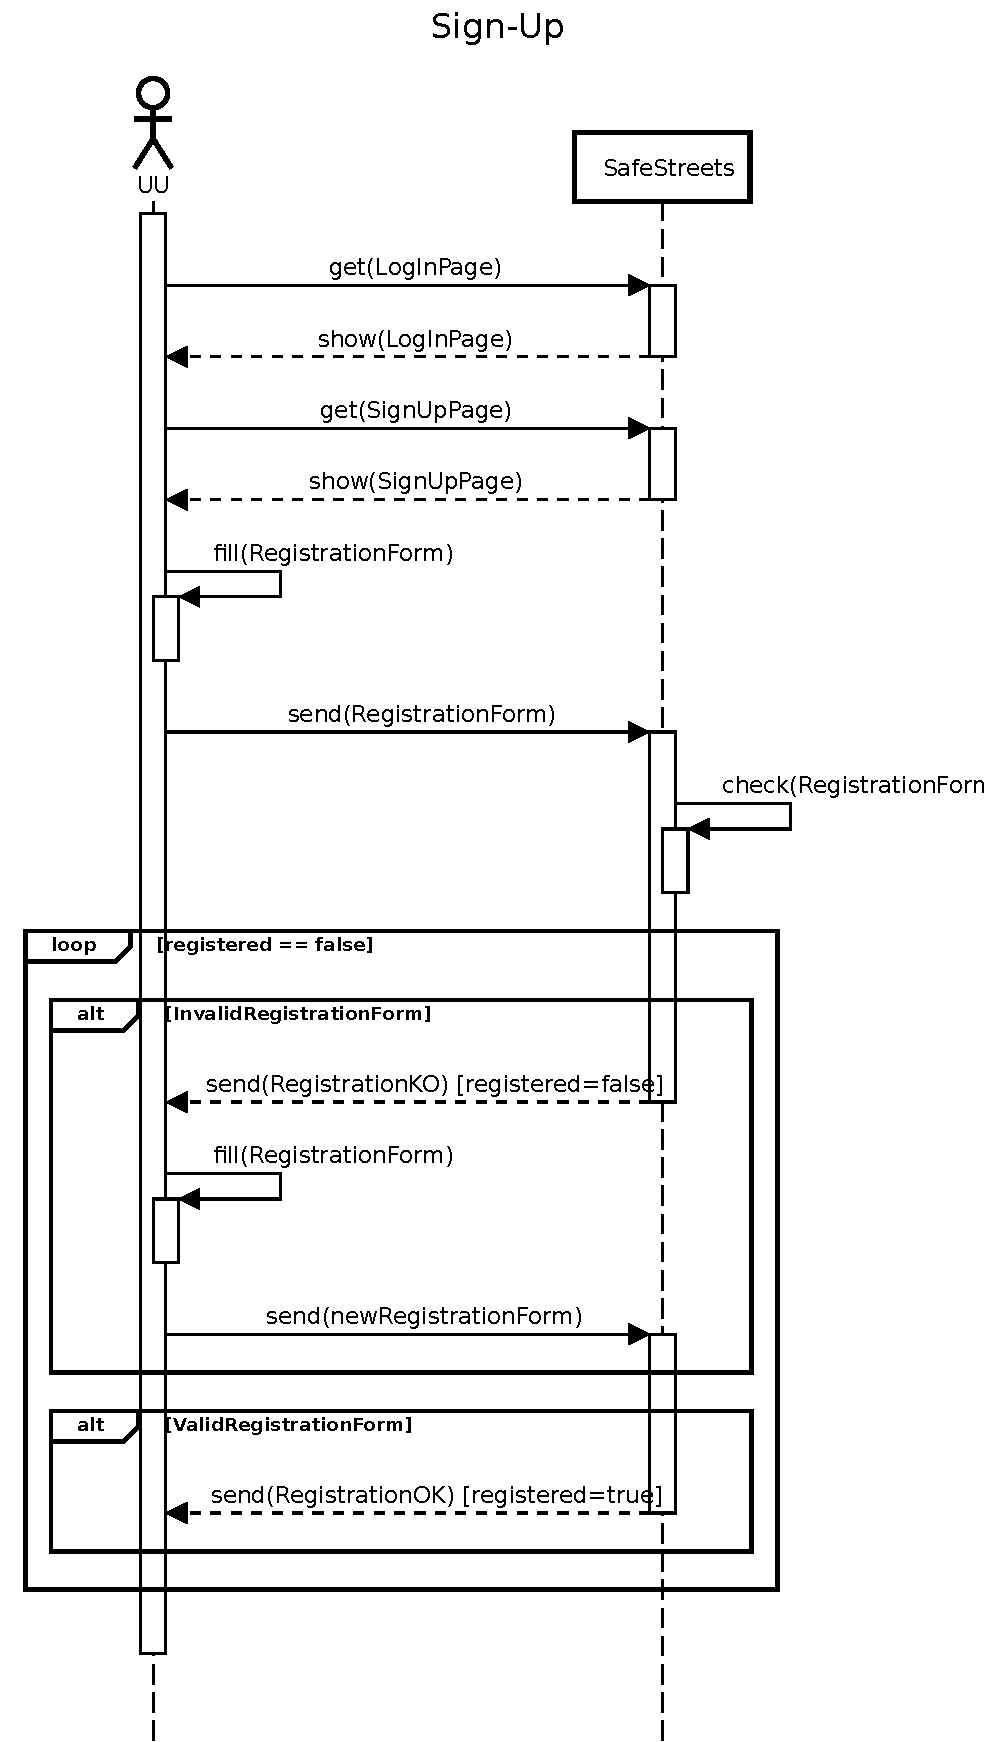
\includegraphics[height=0.85\textheight] {images/SequenceDiagram/SignUp.pdf}
								\caption{UU SignUp sequence diagram}
						\end{figure}
				\subsubsection{Registered User}
					\begin{figure}[!h]
								\centering
							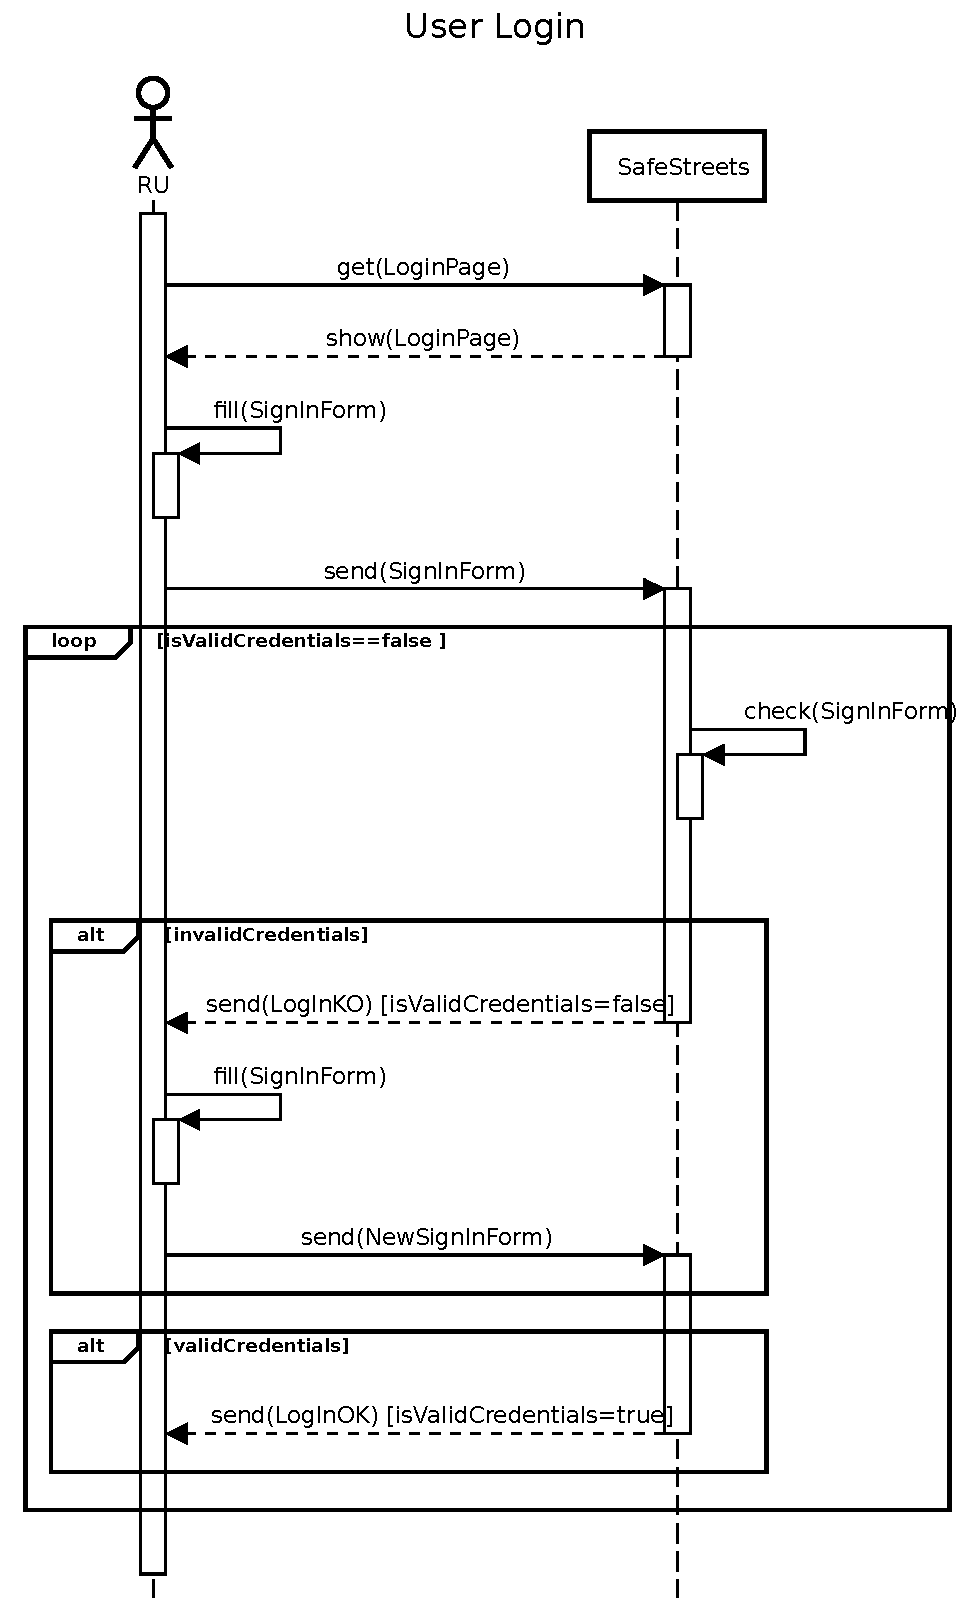
\includegraphics[height=0.8\textheight] {images/SequenceDiagram/User/UserLogIn.pdf}
								\caption{RU LogIn sequence diagram}
						\end{figure}
					\begin{figure}[ht]
								\centering
						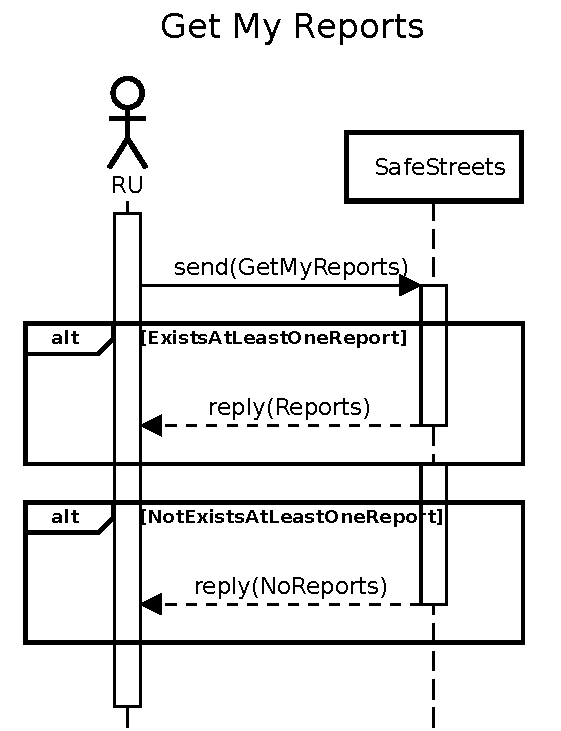
\includegraphics[height=0.4\textheight] {images/SequenceDiagram/User/GetMyReports.pdf}
								\caption{RU Get my reports sequence diagram}
						\end{figure}
					\begin{figure}[!h]
								\centering
							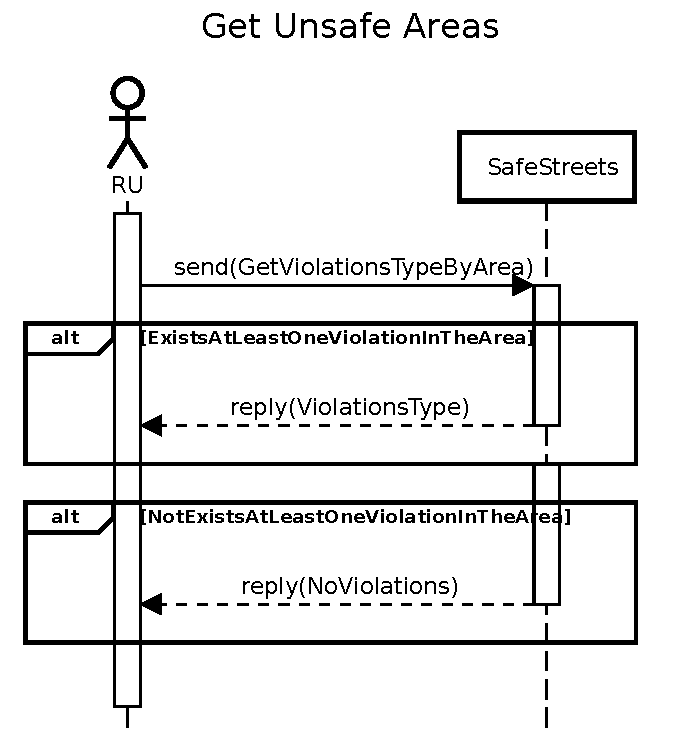
\includegraphics[height=0.4\textheight] {images/SequenceDiagram/User/GetViolationsTypeByArea.pdf}
								\caption{RU Get unsafe areas sequence diagram}
						\end{figure}
					\clearpage
					\begin{figure}[!h]
								\centering
							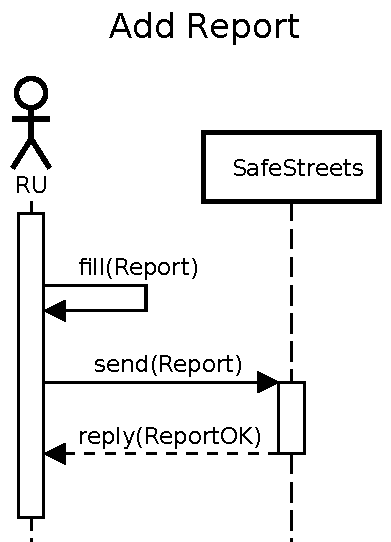
\includegraphics[height=0.5\textwidth] {images/SequenceDiagram/User/AddReport.pdf}
								\caption{RU Add report sequence diagram}
						\end{figure}
					\clearpage
					\subsubsection{Authority}
						\begin{figure}[!h]
								\centering
							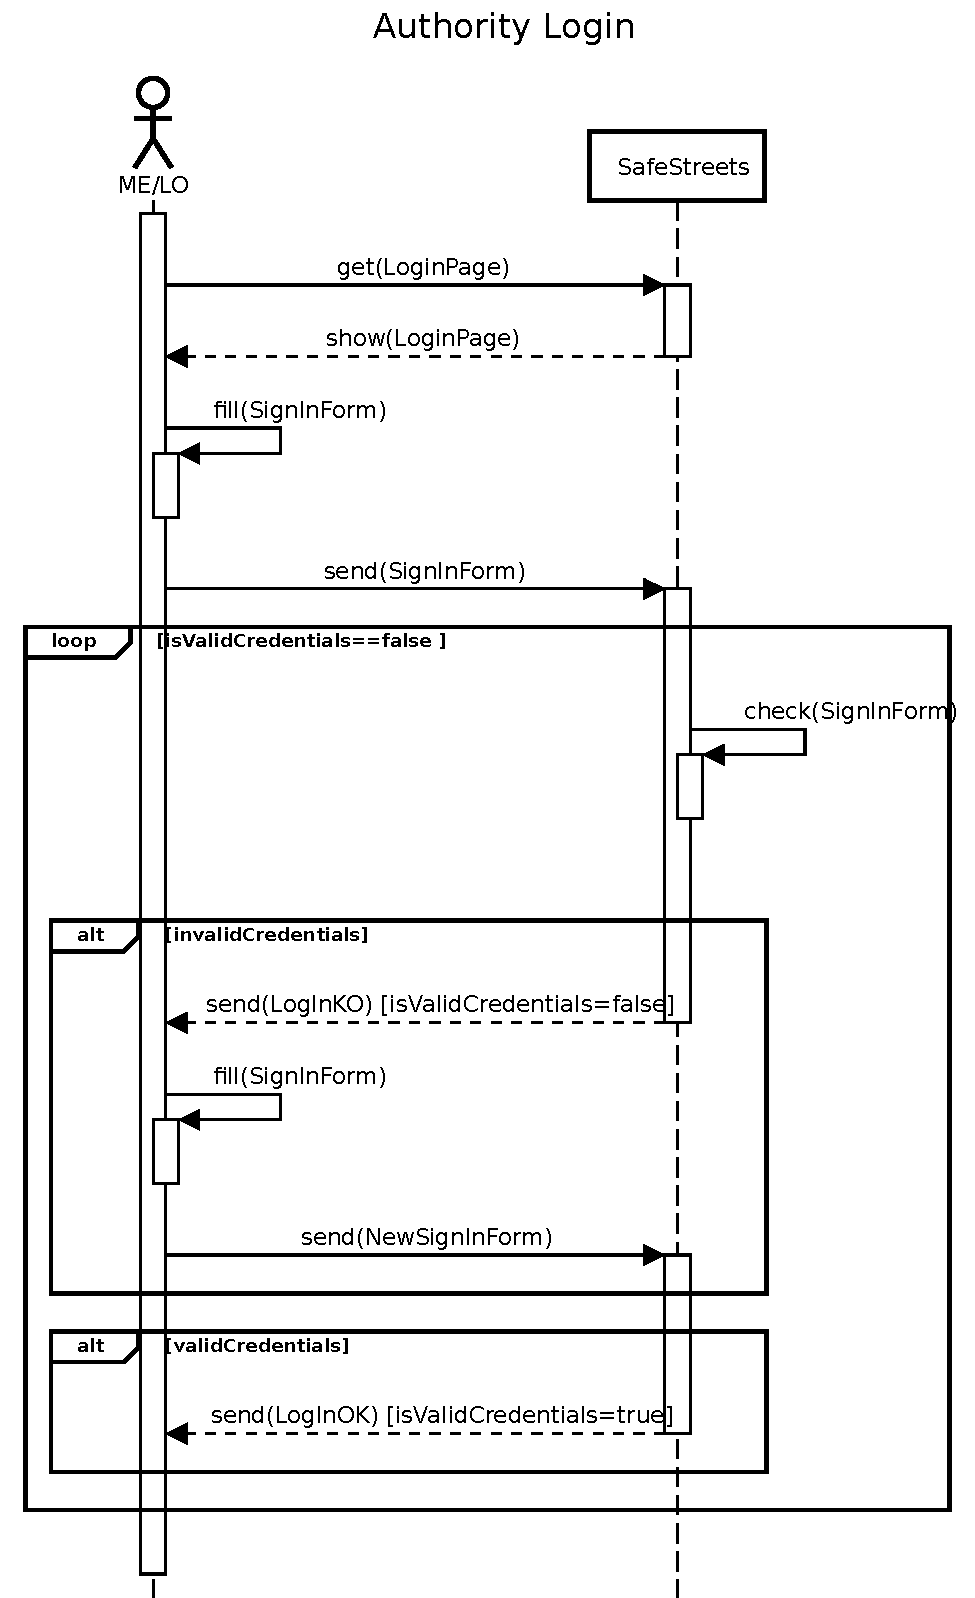
\includegraphics[height=0.8\textheight] {images/SequenceDiagram/Authority/AuthorityLogIn.pdf}
								\caption{Authority LogIn sequence diagram}
						\end{figure}
						\clearpage
						\begin{figure}[!h]
								\centering
							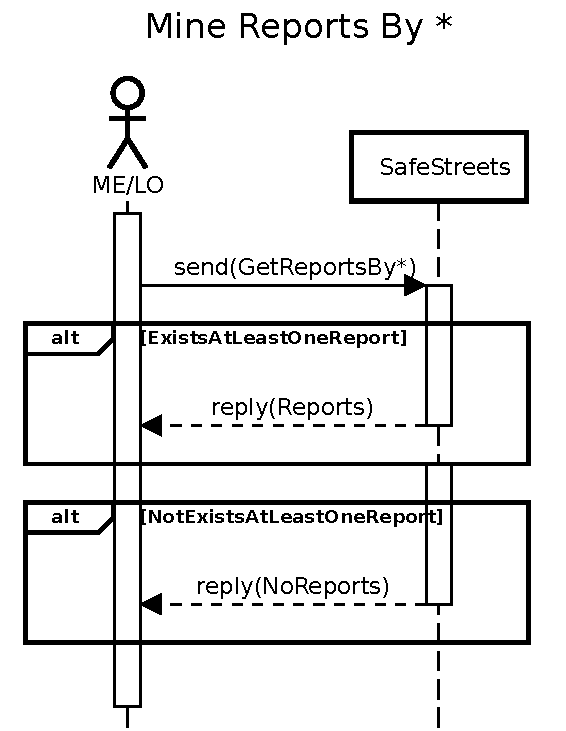
\includegraphics[height=0.4\textheight] {images/SequenceDiagram/Authority/MineReportsBy.pdf}
								\caption{Authority Mine reports by* sequence diagram}
						\end{figure}
						\begin{figure}[!h]
								\centering
							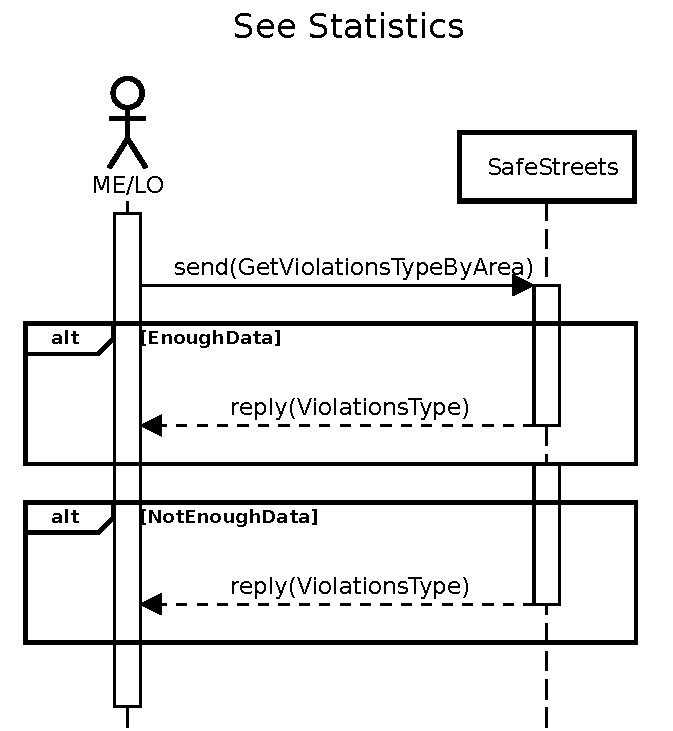
\includegraphics[height=0.4\textheight] {images/SequenceDiagram/Authority/SeeStatistics.pdf}
								\caption{Authority See statistics sequence diagram}
						\end{figure}
					\clearpage
					\subsubsection{Municipal Employee}
						\begin{figure}[!h]
								\centering
							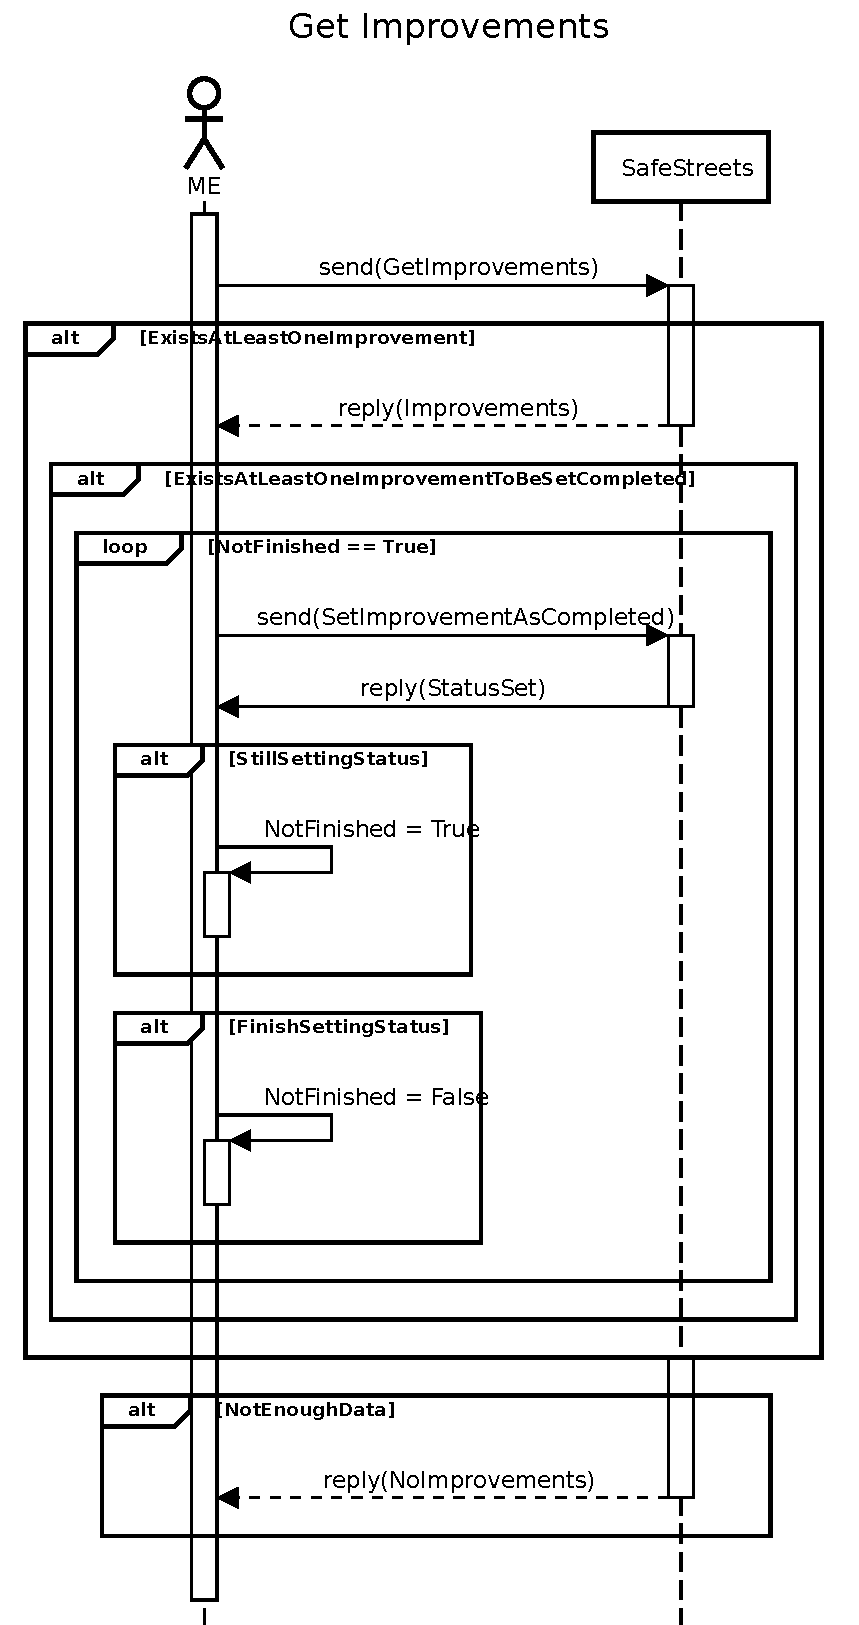
\includegraphics[height=0.5\textheight] {images/SequenceDiagram/Authority/ME/GetImprovements.pdf}
								\caption{Municipal Employee Get improvements sequence diagram}
						\end{figure}
					\clearpage
					\subsubsection{Local Officer}
						\begin{figure}[!h]
								\centering
							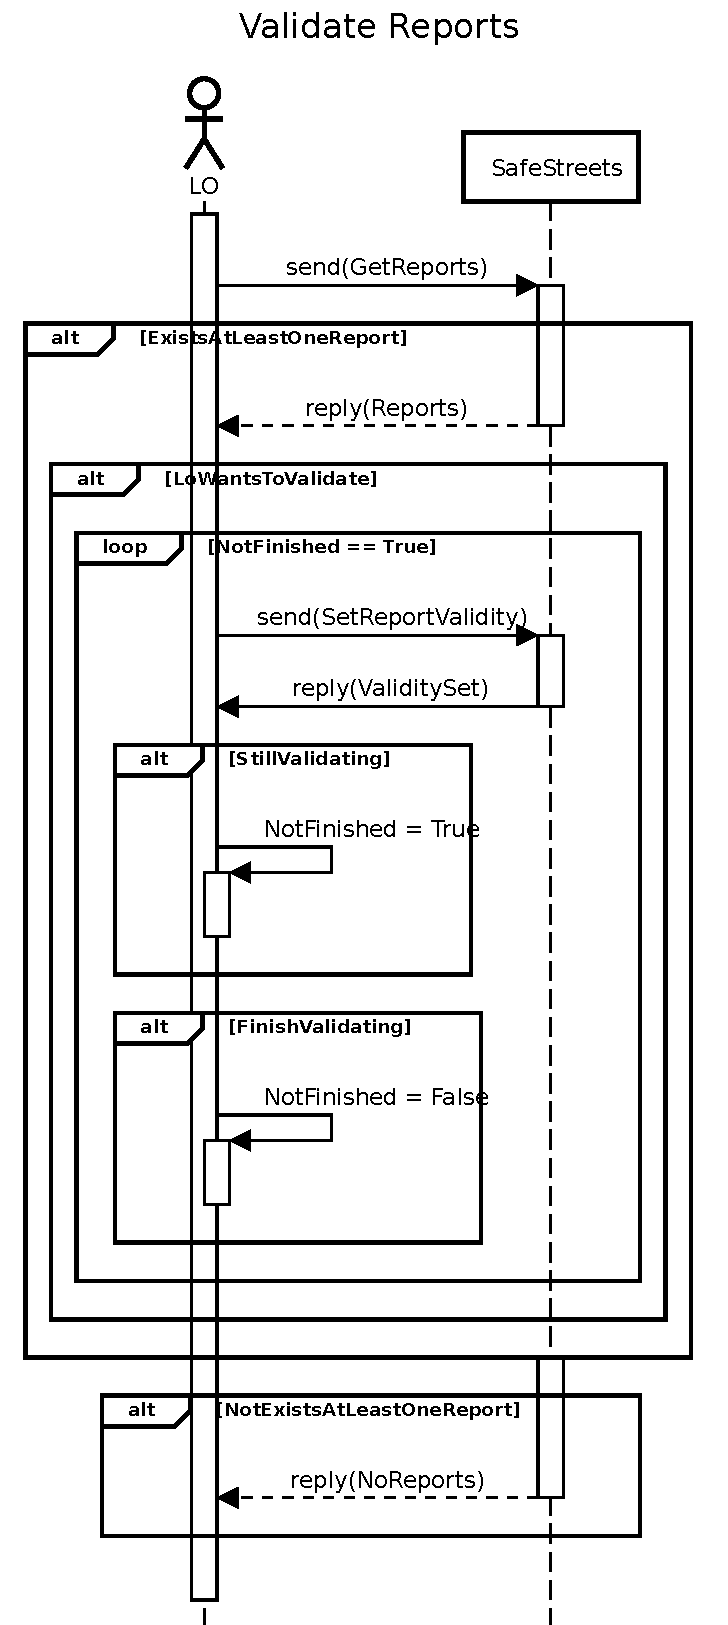
\includegraphics[height=0.8\textheight] {images/SequenceDiagram/Authority/LO/ValidateReport.pdf}
								\caption{Local Officer Validate reports sequence diagram}
						\end{figure}
				\clearpage
				\subsection{Mapping requirements}
					\paragraph{}
						In this section we show that the requirements ensure the satisfaction of the goals in the context of the domain assumptions: the list of requirements and domain assumptions under each goal have this purpose.
					\begin{itemize}
						\item {[G1]} The system must allow logged-in users to send a report of the violation 
							\begin{itemize}
								\item {[D1]} The number of possible violations is finite and is aligned to the current traffic rules
								\item {[D3]} When using the S2B, the user's device is always connected to internet
								\item {[D4]} When using the S2B, the user's device has a valid GPS signal
								\item {[D5]} The internet connection works properly without failure
								\item {[D6]} The user device has a camera and is able to take pictures
								\item {[D7]} The user does not fake his position
								\item {[R1]} A user must be able to sign up to the system with a unique personal username and password
								\item {[R2]} The system must allow only registered users to login with their username and password
								\item {[R4]} A users, municipal employee or local officer must be uniquely identified by his/her username
								\item {[R5]} When composing the report, the system must be able to access the user's device camera and GPS sensor
								\item {[R6]} When composing the report, a user must take a picture from the device's camera and highlight the license plate
								\item {[R7]} When composing the report, time and date get automatically retrieved from the internet 
								\item {[R8]} When composing the report, position gets automatically retrieved from the device's GPS
								\item {[R9]} When composing the report, a user can choose at least one type of violation
								\item {[R10]} When composing the report, a user can't add the same violation type two times in the same report
								\item {[R11]} When composing the report, a user can revert each phase of the creation of the report at any time, before sending it
								\item {[R12]} When composing the report, a user can abort the creation of the report at any time, before sending it
								\item {[R13]} Once a report has been sent, it can't be aborted or reverted
								\item {[R14]} When receiving a report, the system must store it, recognize the car plate, if possible, and marked as unchecked
							\end{itemize}
						\clearpage
						\item {[G2]} The System must allow logged-in users to see their past reports
							\begin{itemize}
								\item {[D3]} When using the S2B, the user's device is always connected to internet
								\item {[D5]} The internet connection works properly without failure
								\item {[R1]} A user must be able to sign up to the system with a unique personal username and password
								\item {[R2]} The system must allow only registered users to login with their username and password
								\item {[R4]} A users, municipal employee or local officer must be uniquely identified by his/her username
								\item {[R15]} When a user asks for his/her reports, the system must provide the saved reports sent by that user
							\end{itemize}
						\item {[G3]} The system must allow logged-in users to retrieve information about the position and types of valid reports
							\begin{itemize}
								\item {[D3]} When using the S2B, the user's device is always connected to internet
								\item {[D4]} When using the S2B, the user's device has a valid GPS signal
								\item {[D5]} The internet connection works properly without failure
								\item {[D7]} The user does not fake his position
								\item {[R1]} A user must be able to sign up to the system with a unique personal username and password
								\item {[R2]} The system must allow only registered users to login with their username and password
								\item {[R4]} A users, municipal employee or local officer must be uniquely identified by his/her username
								\item {[R16]} When getting the valid reports by area, a user can choose a position, or automatically get his/her from the GPS
								\item {[R17]} When getting the valid reports by area, the system must provide all the valid reports near the position given by the user and display their violation type through the MS
							\end{itemize}
						\item {[G4]} The system must allow verified authorities to mine information about date, time, position and type of valid reports
							\begin{itemize}
								\item {[D5]} The internet connection works properly without failure
								\item {[D8]} Every location has one and only one municipality
								\item {[D10]}Each authority has its own account, certified and authorized by a state authority, and linked with the municipality which he/she works for
								\item {[D11]} The official credentials of each municipal employee are different from those used for report violations (if he/she has registered as a normal user)
								\item {[D12]} The official credentials of each local officer are different from those used for report violations (if he/she has registered as a normal user)
								\item {[D13]} The state authority voids credentials of municipal employees or local officers at the end of their service
								\item {[D14]} When using the S2B, the authority's device is always connected to internet
								\item {[R3]} The system must allow only municipal authorities to login with their username and password
								\item {[R4]} A users, municipal employee or local officer must be uniquely identified by his/her username
								\item {[R18]} When mining the information, a municipal employee or a local officer can access only to violations type and date and time of reports occurred in his/her municipality
								\item {[R19]} When mining the information, a municipal employee or a local officer can filter reports by area, date, time or type of violation
							\end{itemize}
						\item {[G5]} The system must allow verified authorities to retrieve statistics about valid reports
							\begin{itemize}
								\item {[D8]} Every location has one and only one municipality
								\item {[D10]}Each authority has its own account, certified and authorized by a state authority, and linked with the municipality which he/she works for 
								\item {[D11]}The official credentials of each municipal employee are different from those used for report violations (if he/she has registered as a normal user)
								\item {[D12]} The official credentials of each local officer are different from those used for report violations (if he/she has registered as a normal user)
								\item {[D13]} The state authority voids credentials of municipal employees or local officers at the end of their service
								\item {[D14]} When using the S2B, the authority's device is always connected to internet
								\item {[R3]} The system must allow only municipal authorities to login with their username and password
								\item {[R4]} A users, municipal employee or local officer must be uniquely identified by his/her username 
								\item {[R21]} When retrieving statistics, a municipal employee or a local officer can access only to reports of violations that occurred in his/her municipality
								\item {[R22]} The system must be able to calculate statistics from the reports of violations and issued tickets of the municipal employee or local officer's municipality
							\end{itemize}
						\clearpage
						\item {[G6]}  The system must be able to cross the data retrieved from the municipality with its own, in order to identify unsafe areas and suggest possible interventions to the municipal employee
							\begin{itemize}
								\item {[D5]} The internet connection works properly without failure
								\item {[D8]} Every location has one and only one municipality
								\item {[D10]} Each authority has its own account, certified and authorized by a state authority, and linked with the municipality which he/she works for
								\item {[D11]} The official credentials of each municipal employee are different from those used for report violations (if he/she has registered as a normal user)
								\item {[D13]} The state authority voids credentials of municipal employees or local officers at the end of their service
								\item {[D14]} When using the S2B, the authority's device is always connected to internet
								\item {[D2]} The number of possible interventions is finite and there exists an already established correlation between violations and possible interventions
								\item {[R3]} The system must allow only municipal authorities to login with their username and password
								\item {[R4]} A users, municipal employee or local officer must be uniquely identified by his/her username
								\item {[R23]} When getting improvements, a municipal employee can access only to data of reports occurred in his/her municipality
								\item {[R24]} The system must be able to retrieve information about accidents from the MAS (municipal accident system)
								\item {[R25]}The system must be able to identify the possible unsafe areas of the municipal employee or local officer's municipality from the reports of violations and data coming the MAS
							\end{itemize}
						\item {[G7]} The system must allow local officer to set the validity of a report sent by the user
							\begin{itemize}
								\item {[D5]} The internet connection works properly without failure
								\item {[D8]} Every location has one and only one municipality
								\item {[D10]} Each authority has its own account, certified and authorized by a state authority, and linked with the municipality which he/she works for 
								\item {[D12]} The official credentials of each local officer are different from those used for report violations (if he/she has registered as a normal user)
								\item {[D13]} The state authority voids credentials of municipal employees or local officers at the end of their service
								\item {[D14]} When using the S2B, the authority's device is always connected to internet
								\item {[R3]} The system must allow only municipal authorities to login with their username and password
								\item {[R4]} A users, municipal employee or local officer must be uniquely identified by his/her username
								\item {[R20]} A local officer must be able to mark a report as valid or not valid
							\end{itemize}
						\item {[G8]} The system must ensure that the chain of custody of the information coming from the user to the municipality is never broken, and the information is never altered
							\begin{itemize}
								\item {[D5]} The internet connection works properly without failure
							\end{itemize}
					\end{itemize}
			\subsection{Traceability matrix}
				\paragraph{}
					The following table keeps track of the relation between Use Cases and Requirements
				\begin{table}[!h]
					\centering
					\begin{tabular}{lL{0.55\textwidth}}
						\toprule
							\textbf{Use cases} & \textbf{Requirements} \\
						\midrule
							Sign-Up & {[R1]} \\
							Registered User login & {[R2]}, {[R4]} \\
							Add Report & {[R5]}, {[R6]}, {[R7]}, {[R8]}, {[R9]}, {[R10]}, {[R11]}, {[R12]}, {[R13]}, {[R14]} \\
							Get My Reports & {[R15]} \\
							Get Violations Type By Area & {[R16]}, {[R17]} \\
							Authority login & {[R3]}, {[R4]} \\
							Get Improvements & {[R23]}, {[R24]}, {[R25]} \\
							See Statistics & {[R21]}, {[R22]} \\
							Mine Reports By Type & {[R18]}, {[R19]} \\
							Mine Reports By Date & {[R18]}, {[R19]} \\
							Mine Reports By Time & {[R18]}, {[R19]} \\
							Mine Reports By Area & {[R18]}, {[R19]} \\
							Validate Reports & {[R20]} \\
						\bottomrule
					\end{tabular}
					\caption{Traceability matrix}
				\end{table}
		\section{Performance requirements}
			\paragraph{}
				The system does not have any particular performance requirements. Obviously, it will have to be able to handle multiple operations from multiple clients (users and authorities) at the same time.
		\section{Design constraints}
			\subsection{Standard compliance}
				\paragraph{}
					The system adopts the current traffic rules in order to provide all the possible VTs.
			\subsection{Hardware limitations}
				\paragraph{}
					The system presents hardware requirements only on the user's side. As a matter of fact, the user is required to have a smartphone with a camera and internet connection (wifi or mobile). Authorities need at least a device capable of connecting to the net.
		\section{Software systems attributes}
			\subsection{Reliability}
				\paragraph{}
					In order to provide reliability, the system must be resilient to faults. The solution is to replicate the system's server. In particular, it will be fault-tolerant against Byzantine faults (faults where a disconnected system has unforeseeable
behaviors) , so the number of replicas of the system's server must be, at least, \textit{(3*number of failing replicas)+1}, with the number of failing replicas decided during the design and implementation.
			\subsection{Availability}
				\paragraph{}
					In order to provide availability, as mentioned in the reliability section, the system's server must be replicated. In this way, it is possible to obtain a 24/7 service. Obviously, little deviations from these requirements will be accepted.
			\subsection{Security}
				\paragraph{}
					In order to provide security, both end users and authorities' data will be always transferred trough encrypted channels. The encryption will be achieved through the usage of public and private keys, each message will be encoded first with the private key of the sender, secondly the public key of the receiver will be used. Moreover every report, sent by the user, is provided with a digital signature, which will make the server able to realize if unauthorized data manipulation has been performed during the data transfer. Thanks to these techniques the purpose of maintaining the chain of custody from the user up to the authorities will be fulfilled.
			\subsection{Maintainability}
				\paragraph{}
					In order to provide maintainability, the development of the system has to be done so that will be easy and cheap to fix and modify it in the future. In order to achieve these properties, appropriate design patterns will be used. More of this in the design document.
			\subsection{Portability}
				\paragraph{}
					In order to provide portability, the system will be available as a downloadable app for the user and as a web service for the authorities.